\documentclass[english, a4paper]{article}

%for writing
\usepackage{lmodern}
\usepackage[utf8]{inputenc}
\usepackage[T1]{fontenc}
\usepackage{babel}

%for layout
\usepackage[
    a4paper,
    left=25mm,
    right=25mm,
    top=25mm,
    bottom=25mm
    ]{geometry}

% for maths
\usepackage{amsmath}
\usepackage{amsfonts}
\usepackage{amssymb}
\usepackage{amsthm}

%for graphics
\usepackage{graphicx}
\usepackage{subcaption}

%for tables
\usepackage{array}

% for refs (in that order)
\usepackage{hyperref}

% for headers and footers
\usepackage{fancyhdr}

% For collaboration
\usepackage{easyReview}

% For acronyms and index
\usepackage{glossaries}

% Custom commands
\usepackage{import}

\theoremstyle{plain}
\newtheorem{prop}{Proposition}

\theoremstyle{definition}
\newtheorem{definition}{Definition}

\theoremstyle{remark}
\newtheorem{remark}{Remark}

\newcommand{\keywords}[1]
{
    \small
    \textbf{Keywords:} #1
    \vspace{0.2cm}
}

\import{}{accronyms.tex}

%document properties
\title{High Occupancy Vehicle Lane and Metro-like Carpooling. A Bottleneck Case Study}

\author{Martin Briand$^{a,}$\footnote{Martin Briand is the corresponding author. His corresponding email is \href{mailto:martin.briand23@gmail.com}{martin.briand23@gmail.com}}, Nicolas Coulombel$^{b}$, Guillaume Monchambert$^{c}$\\
\small $^{a}$Martin’s affiliation\\
\small $^{b}$Nicolas’ affiliation\\
\small $^{c}$Guillaume’s affiliation}

\date{2025}

% document
\begin{document}

\maketitle

\begin{abstract}
    No abstract
\end{abstract}

\keywords{No keywords for the moment…}
\alert{TODO} % TODO keywords

\clearpage
\part{Article}

\section{Introduction}
\alert{TODO} % TODO Introduction

\section{Literature Review}
\alert{TODO} % TODO Literature Review

\section{Model}
\subsection{Traffic technology}

We consider a single highway linking a residential location and a \acrfull{cbd} where people work. Every day, some commuters from the residential area go to the \acrshort{cbd}. The capacity of the highway is shared between a \acrfull{rl} and a \acrfull{gpl}. In addition, at the beginning and end of the road, there are two carpooling stations. At the upstream station, carpooling passengers can safely get in drivers' car on \acrshort{rl}. These same passengers will then safely alight at the downstream station. Travelers can choose between driving alone on the \acrshort{gpl} (their corresponding variables will be denoted by the subscript letter $s$ for ``solo''), drive on the \acrshort{rl} while being forced to take all passengers that would be waiting at the upstream station when they pass it, if any, up to the capacity of their vehicle (their corresponding variables will be denoted by the subscript letter $d$ for ``driver''), or be a carpooling passenger and wait at the carpooling station until some carpooling driver arrive at the station to pick them up (their corresponding variables will be denoted by the subscript letter $p$ for ``passenger'').

In a bottleneck fashion, the highway has a capacity $s$ (not to be mistaken for the subscript of solo-drivers). $\varphi$ denotes the share of the reserved capacity. \acrshort{rl} hence has a capacity of $\varphi s$ and \acrshort{gpl} a capacity of $(1-\varphi)s$. Denoting $T_f$ the free-flow travel time (common between the two lanes), $T_s(t)$ and $T_d(t)$ the travel time of a driver departing at $t$ on the \acrshort{gpl} and the \acrshort{rl} respectively, we can define $T^{\nu}_s(t)$ and $T^{\nu}_d(t)$ the respective times lost in congestion as $T^{\nu}_i(t) = T_i(t) - T_f$ where $i$ is either $s$ or $d$. We suppose that the congestion occurs vertically right before the downstream station. Then, defining $r_s (t)$ and $r_d (t)$ as the respective incoming flows of solo-drivers and carpooling drivers at the beginning of the road (which is not disturbed by congestion due to the vertical queue hypothesis), and given any set of initial conditions $T^{\nu}_i(\bar{t}_i) \geq 0$, $T^{\nu}_i$ are uniquely defined by the differential equations:

\begin{equation}
    \frac{d T^{\nu}_i(t)}{dt} s_i = \left\{
    \begin{array}{lr}
        r_i (t) - s_i & \text{if } T^{\nu}_i(t) > 0\\
        \max (0, r_i (t) - s_i) & \text{if } T^{\nu}_i(t) = 0
    \end{array}
    \right.
\end{equation}
where $s_d = \varphi s$ and $s_s = (1-\varphi)s$.

As for the carpooling passengers at the upstream station, they can also queue at the station in a bottleneck fashion. Denoting $r_p(t)$ the arrival rate of passengers at the upstream station, $M$ the capacity of passengers in vehicles without the driver (for example $M=3$ if all vehicles are small cars with 4 seats), $q^{\nu}_p(t)$ the number of passengers waiting at the station at time $t$, and given an initial condition $q^{\nu}_p(\bar{t}_p) \geq 0$, $q^{\nu}_p$ is uniquely defined by the differential equation below:

\begin{equation}
    \label{eq_queue_at_station}
    \frac{d q^{\nu}_p(t)}{dt} = \left\{
    \begin{array}{lr}
        r_p (t) - M r_d (t) & \text{if } q^{\nu}_p(t) > 0\\
        \max (0, r_p (t) - M r_d (t)) & \text{if } q^{\nu}_p(t) = 0
    \end{array}
    \right.
\end{equation}

Then, we can define $T^{\nu}_p(t)$ the time elapsed between an arrival at the station at time $t$ and the departure from that station supposing a \acrfull{fifo} queuing method as:

\begin{itemize}
    \item if $q_p^{\nu}(t) = 0$, then $T^{\nu}_p(t) = 0$
    \item else
    \begin{itemize}
        \item if there is no $T^{\nu}_p \geq 0$ such that $M \times \int_{t}^{t+T^{\nu}_p} r_d(t) dt \geq q_p^{\nu}(t)$, then $T^{\nu}_p(t) = +\infty$
        \item else, $T^{\nu}_p(t)$ is the smallest $T^{\nu}_p \geq 0$ such that $M \times \int_{t}^{t + T^{\nu}_p} r_d(t') dt' \geq q_p^{\nu}(t)$
    \end{itemize}
\end{itemize}

Finally, we define the travel time of a carpooling passenger arriving at the station at $t$ as the sum of the time spent waiting at the station and the travel time, namely $T_p(t) = T^{\nu}_p(t) + T_d(t + T^{\nu}_p(t)) = T^{\nu}_p(t) + T^{\nu}_d(t + T^{\nu}_p(t)) + T_f$.


\subsection{Population and costs}

We suppose that we have a fixed demand of $N$ commuters. All of these commuters wish to arrive at the same desired arrival time $t^*$. By choosing a mode $i\ \in \left\{ s, d, p \right\}$ and a departure time $t$, they experience a travel time cost $\alpha \times T_i(t)$ (which will be shortened as $\text{tt}_i$) where $\alpha$ is the shadow value of travel time. They also experience a delay cost $\max [\beta \times (t^* - (t + T_i(t))), \gamma \times ((t + T_i(t)) - t^*)]$ (which will be shortened as $\text{sched}_i(t)$) where $\beta$ and $\gamma$ are the respective shadow values of time early and late. As usual in bottleneck formulations, we suppose $0 < \beta < \alpha$ and $0 < \gamma$. 

Every driver, either $s$ or $d$, also experiences a cost $f$ to operate their car that represents the cost of energy (hence the letter $f$ for ``fuel'') but also wear and tear costs, insurance cost, repair costs... All externalities due to car use but congestion are represented by the cost $E$ (for ``externality''). These are not experienced by drivers when choosing their mode, but are included in social cost functions. This could represent the sum of safety, air quality and environmental externalities for example.

The drivers of the reserved lanes are supposed to be insensitive to the expected probability of having passengers. By proposing their seats (whether there are passengers seated on them or not), they experience the potentially negative inconvenience cost $\overline{\Delta_d}$ \footnote{The fact that $\overline{\Delta_d}$ is independent of the probability of the driver to embark passengers is unrealistic. Of course, if it was certain that no commuter ever choose the passenger mode, drivers would be indifferent between offering their seats or not for they would know that their offer is nothing but virtual. We will see however that this unrealistic case only occurs with unrealistic values, and that this simplifying hypothesis is not much of a problem when interpreting the results}.

Similarly, carpooling passengers experience an inconvenience cost $\Delta _p$. However, opposite to carpooling driver inconvenience cost, this cost is distributed in the population according to the cumulative distribution function $F$. For example, there are $N \times F(\Delta _p ^0)$ commuters whose $\Delta _p$ value is lower than $\Delta _p ^0$. We also suppose that the values of $\Delta _p$ are bounded and that these bounds are reached. That is to say that there is at least one commuter whose passenger inconvenience cost is $\Delta _p ^{\text{min}}$ and $\Delta _p^{\text{min}} \leq \Delta _p$ for all other commuters. Similarly, there is at least one commuter whose passenger inconvenience cost is $\Delta _p ^{\text{max}}$ and $\Delta _p^{\text{max}} \geq \Delta _p$ for all other commuters. We also suppose that:
\begin{itemize}
    \item $F$ is continuous, differentiable, and strictly increasing,
    \item The density function which is the derivative of $F$ and denoted $F'$ is well-defined, continuous and positive.
    \item $F^{-1} := [0, 1] \longrightarrow [\Delta_p^{\text{min}}, \Delta_p^{\text{max}}]$ the invert of $F$ is well-defined, continuous and differentiable.
    \item The derivative of $F^{-1}$, $(F^{-1})^{'} = \frac{1}{F'\circ F^{-1}}$ is well-defined, positive and continuous.
\end{itemize}

Finally, carpooling drivers and passengers both have to pay a (potentially negative) fare for choosing their mode. This fare can be time-dependent. A carpooler choosing mode $i \in \left\{ p, d \right\}$ and departing at time $t$ would have to pay a fare $\rho _i (t)$.

To summarize, a commuter with a given $\Delta _p$ value will experience the following costs depending on the mode she chooses:

\begin{equation}
\left\{
\begin{array}{l}
    c_s(t) = \text{tt}_s(t) + \text{sched}_s(t) + f\\
    c_d(t) = \text{tt}_d(t) + \text{sched}_d(t) + f + \overline{\Delta _d} + \rho _d (t)\\
    c_p(t) = \text{tt}_p(t) + \text{sched}_p(t) + \Delta _p + \rho _p (t)
\end{array}
\right.
\end{equation}
% introducing an equation is introducing a bias. don’t forget to say it.

Her contribution to social cost will be:
\begin{equation}
    \left\{
    \begin{array}{l}
        sc_s(t) = c_s(t) + E\\
        sc_d(t) = c_d(t) + E - \rho _d (t)\\
        sc_p(t) = c_p(t) - \rho _p(t)
    \end{array}
    \right.
\end{equation}

The organizer of the carpooling service will experience a profit (potentially negative) of:

\begin{equation}
    \int_{\text{time}} (r_p(t) \rho _p(t) + r_d(t) \rho _d(t)) dt
\end{equation}

Without loss of generality, we can suppose that $T_f = 0$ and that there is no queue before the first commuter arrives, either on the road or at the upstream carpooling station.


\subsection{Equilibria for time-independent fares}

Suppose we have an equilibrium between the three modes, we denote $N_s$, $N_d$ and $N_p$ the number of commuters choosing the solo-driver, carpooling driver and carpooling passenger modes respectively. These help variables are subject to the following constraints: $N_s + N_d + N_p = N$, $0 \leq N_s = \int_{\text{time}} r_s(t) dt$, $0 \leq N_d = \int_{\text{time}} r_d(t) dt$ and $0 \leq N_p = \int_{\text{time}} r_p(t) dt$.

We also suppose that fares are time-independent. This assumption will be relaxed later, but since it is a plausible constraint on fare policies to be time-independent, we first try to understand equilibria under such a constraint. We hence rewrite $\rho _d(t)$ as $\rho _d$ and $\rho _p(t)$ as $\rho _p$.

\subsubsection{For $\varphi = 0$}

The problem is trivial since everyone commutes as a solo driver and the problem reduces to a simple bottleneck problem.

We have $N_d = N_p = 0$ and $N_s = N$.

\begin{equation}
\label{eq_rs}
r_s(t) = \left\{
\begin{array}{lr}
    0 & \text{if } t<t_s^0\\
    s\left( 1 + \frac{\beta}{\alpha - \beta} \right) & \text{if } t_s^0 \leq t < \tilde{t}_s\\
    s\left( 1 - \frac{\gamma}{\alpha + \gamma} \right) & \text{if } \tilde{t}_s \leq t \leq t_s^1\\
    0 & \text{if } t_s^1 < t
\end{array}
\right.
\end{equation}
where

\begin{equation}
\label{eq_ts}
\left\{
\begin{array}{l}
    t_s^0 = t^* - \frac{N_s}{s} \times \frac{\gamma}{\beta + \gamma}\\
    \tilde{t}_s = t^* - \frac{N_s}{s} \times \frac{\beta \gamma}{\alpha(\beta + \gamma)}\\
    t_s^1 = t^* + \frac{N_s}{s} \times \frac{\beta}{\beta + \gamma}
\end{array}
\right.
\end{equation}

Writing $\delta = \frac{\beta \gamma}{\beta + \gamma}$, the cost experienced by each commuter is $\frac{\delta N}{s} + f$ and the total social cost is $\frac{\delta N^2}{s} + N(E + f)$. The profit of the organizer is $0$.

\subsubsection{For $\varphi = 1$}

We have $N_s = 0$ and everybody carpools.

\begin{definition}[Feasible modal split]
    A modal split $(N_d, N_p)$ is said to be feasible if $0 \leq N_p \leq M \times N_d$ and $N_p + N_d = N$.    
\end{definition}

\begin{remark}
    It is easy to note that this definition is equivalent to $N_d \geq N \times \frac{1}{1+M}$, $N_p \geq 0$ and $N_p + N_d = N$.
\end{remark}

For some given $\rho_d$ and $\rho_p$, suppose there is an equilibrium with $N_d \geq 0$ drivers and $N_p \geq 0$ passengers. Clearly, since having more passengers than car capacity would lead to infinite cost for some passengers, it is clear that an equilibrium should lead to a feasible modal split.

Since the cost function experienced by drivers is independent of the behavior of passengers, they spread across time according to the classic bottleneck model:

\begin{equation}
\label{eq_rd}
r_d(t) = \left\{
\begin{array}{lr}
    0 & \text{if } t<t_d^0\\
    s\left( 1 + \frac{\beta}{\alpha - \beta} \right) & \text{if } t_d^0 \leq t < \tilde{t}_d\\
    s\left( 1 - \frac{\gamma}{\alpha + \gamma} \right) & \text{if } \tilde{t}_d \leq t \leq t_d^1\\
    0 & \text{if } t_d^1 < t
\end{array}
\right.
\end{equation}
where

\begin{equation}
\label{eq_td}
\left\{
\begin{array}{l}
    t_d^0 = t^* - \frac{N_d}{s} \times \frac{\gamma}{\beta + \gamma}\\
    \tilde{t}_d = t^* - \frac{N_d}{s} \times \frac{\beta \gamma}{\alpha(\beta + \gamma)}\\
    t_d^1 = t^* + \frac{N_d}{s} \times \frac{\beta}{\beta + \gamma}
\end{array}
\right.
\end{equation}

They experience a cost of $\frac{\delta N_d}{s} + f + \overline{\Delta _d} + \rho _d$ and their contribution to total social cost is $\frac{\delta N_d^2}{s} + N_d(E + f) + N_d \overline{\Delta _d}$.

As for passengers, it is slightly more complicated. First, we note that a commuter departing at $t$ with passenger inconvenience cost $\Delta _p$ and choosing to be passenger experiences a cost $\frac{\delta N_d}{s} + \rho _p + \Delta _p + T^{\nu}_p(t)$. Then sorting commuters by $\Delta _p$, either the one with the lowest passenger inconvenience cost does not see any interest in being passenger, and there are only drivers, or there is some commuter whose inconvenience cost is $\Delta _p^{\text{switch}}$ and who is indifferent between driving and being a passenger.

We define $\Delta _p^{\text{full}} = F^{-1}\left( \frac{M}{1+M} \right)$, the threshold beyond which it is physically impossible to make more drivers switch to passengers due to vehicle capacity limit. This help variable being defined, we now study three cases:

\begin{itemize}
    \item If $\Delta _p^{\text{min}} \geq f + \overline{\Delta _d} + \rho _d - \rho _p$, then there are no carpooler and everyone drives. This is the only equilibrium.
    
    \item If there exist a $\Delta _p^{\text{switch}} \in ]\Delta _p^{\text{min}}, \Delta _p^{\text{full}}[$ such that $\Delta _p^{\text{switch}} = f + \overline{\Delta _d} + \rho _d - \rho _p$. Then, due to the fact that $T^{\nu}_p(t) \geq 0$ for all $t$, an equilibrium could no involve more than $N\times F(\Delta _p^{\text{switch}})$ passengers. Then, since $N_p < MN_d$, some drivers have some empty seats, and Equation \ref{eq_queue_at_station} tells us that there is no queue at the station for passengers when these drivers pass it. Therefore, for every $r _p(t)$, if there is a $t$ for which $q(t) > 0$ and $r_p(t) > 0$, then the passengers departing at $t$ could depart with the drivers in question and experience no queue and a lower cost. In other words, an equilibrium necessarily involves a passenger inflow function $r_p(t)$ that satisfies $r_p(t) \leq M r_d(t)$ for all $t$ and $r_p(t) = 0$ when $r_d(t) = 0$. Such a function implies no queue for passengers ($T^{\nu}_p (t) = 0$ for all $t$). Using this, it is straightforward to see that all commuters with passenger inconvencience cost lower than $\Delta _p^{\text{switch}}$ are passengers, those whose passenger inconvenience cost is larger are drivers, and the one whose inconvencience cost is $\Delta _p^{\text{switch}}$ is indifferent between the two modes. Finally, noticing that all splits with $N_p = N\times F(\Delta _p^{\text{switch}})$ and $r_p(t)$ as defined above are equilibria, this finishes the characterization of equilibria for that case.
    
    \item If $\Delta _p^{\text{full}} \leq f + \overline{\Delta _d} + \rho _d - \rho _p$. Having strictly less than $\frac{M}{M+1}$ passengers would always lead to some empty seats in drivers’ cars with no queue for passengers due to Equation \ref{eq_queue_at_station}. As a consequence, some drivers with passenger inconvenience cost strictly lower than $\Delta _p^{\text{full}}$ would have an interest in switching to passenger, and subsequently, equilibrium could only involve $N_p = \frac{M}{M+1} = F(\Delta _p^{\text{full}})$ passengers. In a similar way, it is impossible to have an equilibrium in which two commuters $a$ and $b$ with respective carpooling inconvenience costs $\Delta_p^a < \Delta_p^b$ are respectively driver and passengers. As a matter of facts, if commuter $b$ were to prefer the passenger mode and depart at time $t$, by choosing to depart right before commuter $b$, commuter $a$ would indeed incur a strictly lower cost than commuter $b$, whose cost was already lower than commuter $a$’s when he was a driver. Therefore, an equilibrium necessarily means that all commuters with $\Delta _p \leq \Delta _p^{\text{full}}$ are passengers and others drive. Moreover, it should be the case that passengers are indifferent in choosing when to depart among all departure times. Therefore, $T^{\nu}_p(t)$ should be constant for all $t$ where $r_p(t) > 0$. We write it $T^{\nu}_p$. Furthermore, since at equilibrium, all drivers experience the same cost, and since, up to the inconvenience cost, all passengers experience the same cost, and since one commuter should be indifferent between passenger and driver, the only commuter that could be indifferent is the one with $\Delta _p = \Delta_p^{\text{full}}$. We hence find $T^{\nu}_p = \frac{1}{\alpha} (f + \overline{\Delta _d} - \Delta _p ^{\text{full}} + \rho _p - \rho _d)$. Then, the definition of $T^{\nu}_p$ gives $q_p^{\nu}(t) = M\times \int _t^{t+ T^{\nu}_p} r_d(t') dt'$ for all $t$ such that $r_p(t) >0$. Deriving this equation, we get $\frac{dq_p^{\nu}(t)}{dt} = M\times [r_d(t + T_p^{\nu}) - r_d(t)]$. Since no seat capacity can be wasted (or some passenger would have an infinite cost), it is impossible to have $q_p^{\nu}(t) = 0$ and $r_p(t) < Mr_d(t)$ at the same time. Therefore, Equation \ref{eq_queue_at_station} gives $\frac{dq_p^{\nu}(t)}{dt} = r_p(t) - Mr_d(t)$. And finally, $r_p(t) = Mr_d(t+ T^{\nu}_p)$.

    Said otherwise, the only potential equilibrium is a modal split with $\frac{1}{M+1}$ drivers and $\frac{M}{M+1}$ passengers. The commuter whose passenger inconvenience cost is $\Delta _p^{\text{full}}$ is indifferent between the two modes, those whose passenger inconvenience cost is lower are passengers, and those for whom it is larger are drivers. Drivers depart according to a classic bottleneck model, and passengers follow the departure rate of drivers, scaled by a factor $M$, and with an advance of $T^{\nu}_p = \frac{1}{\alpha} (f + \overline{\Delta _d} - \Delta _p ^{\text{full}} + \rho _p - \rho _d)$. But if $T^{\nu}_p > 0$, this only candidate for equilibrium is not an equilibrium since the passenger departing last would have an interest in departing right at the departure time of the last driver to get in the same car, enjoy the same travel time on road, but without queue at the station. It is therefore impossible to have an equilibrium if $\Delta _p^{\text{full}} < f + \overline{\Delta _d} + \rho _d - \rho _p$.
\end{itemize}

This leads us to the following property.

\begin{prop}
    \begin{itemize}
        \item For any given fare policy $(\rho_d, \rho_p)$:
        \begin{itemize}
            \item If $\Delta _p^{\text{full}} < f + \overline{\Delta _d} + \rho _d - \rho _p$, there is no equilibrium.
            \item Else, there exists a unique feasible modal split $(N_d, N_p)$ which is an equilibrium. If the unique feasible modal split is either $(N_p = 0, N_d = N)$ or $(N_p = \frac{M}{M+1}, N_d = \frac{1}{M+1})$, then the time distribution of passengers is uniquely determined, otherwise, it is not.
        \end{itemize}
    
        \item And for any feasible modal split $(N_d, N_p)$, there exists some (non-unique) fare policy $(\rho _d, \rho _p)$ such that $(N_d, N_p)$ is the unique feasible modal split which is a resulting equilibrium. Especially, if $N_p > 0$, then the difference $\rho _p - \rho _d$ is unique. If $N_p = 0$ or $N_p = N\times \frac{M}{M+1}$, the time distribution of passengers is uniquely determined. It is however not possible to choose the time distribution of passengers if $0 < N_p < MN_d$.
    \end{itemize}
\end{prop}

\begin{proof}
    The first part of the proposition is already proven above.

    For the second part, it is straightforward to notice that:
    \begin{itemize}
        \item if $N_p = 0$ and $N_d = N$, then, then any $\rho _p$ and $\rho _d$ satisfying $\rho _p - \rho _d \geq f + \overline{\Delta _d} - \Delta _p^{\text{min}}$ is solution;
        \item if $0 < N_p < N \times \frac{M}{M+1}$, then defining $\Delta _p^{\text{switch}} = F^{-1}\left(\frac{N _p}{N} \right)$, any $\rho _p$ and $\rho _d$ satisfying $\rho _p - \rho _d = f + \overline{\Delta _d} - \Delta _p^{\text{switch}}$ is solution.
        \item if $N_p = N \times \frac{M}{M+ 1}$ and $N_d = N \times \frac{1}{M+ 1}$, then any $\rho _p$ and $\rho _d$ satisfying $\rho _p - \rho _d = f + \overline{\Delta _d} - \Delta _p^{\text{full}}$ is solution.
    \end{itemize}
    
\end{proof}

To get a good grasp of how drivers and passengers distributes in time, Figure \ref{fig_arrival_rates} presents cumulative departures (solid lines) and arrivals (dashed) for the three regimes. One can note that the case where $\Delta_p^{\text{full}} < f + \overline{\Delta_d} + \rho_d - \rho_p$ is not presented for it leads to no equilibrium.

For all regimes, drivers have the very standard bottleneck departure rates (see Subfigure \ref{subfig_arrival_rates_no_passenger} for slope equations) and arrival rates ($s$). However, the distances of $t_d^0$, $\tilde{t}_d$ and $t_d^1$ relative to $t^*$ are proportional between figures, but smaller as the red dot moves to the right or as the number of drivers decreases. A more graphic interpretation is to say that as we progress toward higher average filling rates, the x-axis are zoomed-in with a zoom ratio that is the inverse of the $N_d / N$ proportion indicated in the titles of the subfigures.

For passengers however, while having one unique departure ratio for the two extreme cases (no passenger, full utilization of vehicles’ capacity), Subfigure \ref{subfig_arrival_rates_interior} presents only two examples of passengers arrival rate, both starting with the first driver, but we could imagine infinitely more, the two only rules being that $r_p(t) \leq Mr_d(t)$ at all times and the all the $N_p$ passengers should depart.

\begin{figure}
\begin{center}
    \begin{subfigure}{.32\textwidth}
    \begin{center}
        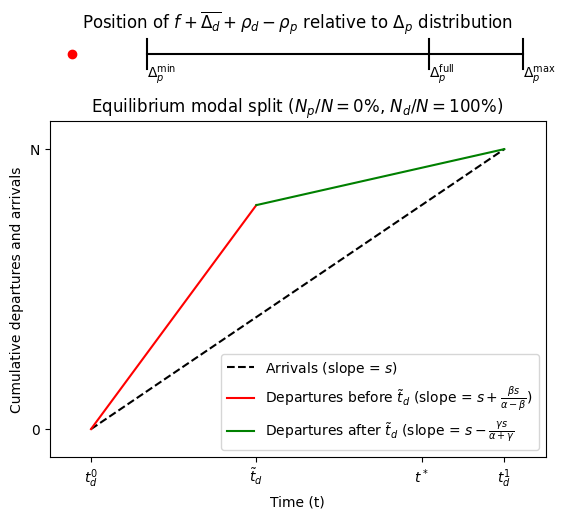
\includegraphics[width=\textwidth]{images/arrivals1.png}
        \caption{No passenger: equilibrium is unique}
        \label{subfig_arrival_rates_no_passenger}
    \end{center}
    \end{subfigure}% this comment has to be here to avoid vertical stacking of figures
    \hfill
    \begin{subfigure}{.32\textwidth}
    \begin{center}
        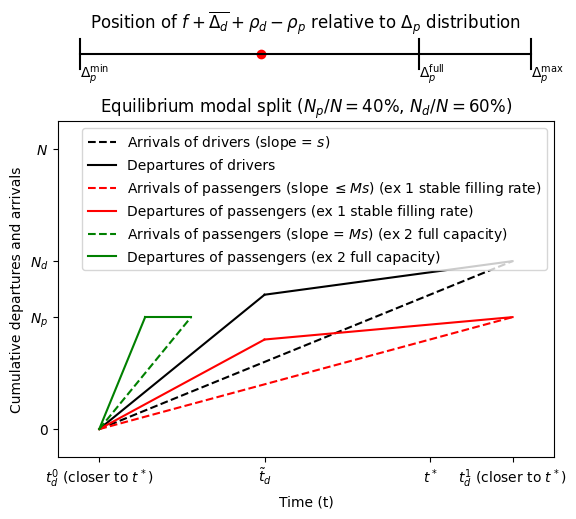
\includegraphics[width=\textwidth]{images/arrivals2.png}
        \caption{Partial utilization of car capacity: equilibrium is unique for drivers and infinite for passengers}
        \label{subfig_arrival_rates_interior}
    \end{center}
    \end{subfigure}% this comment has to be here to avoid vertical stacking of figures
    \hfill
    \begin{subfigure}{.32\textwidth}
    \begin{center}
        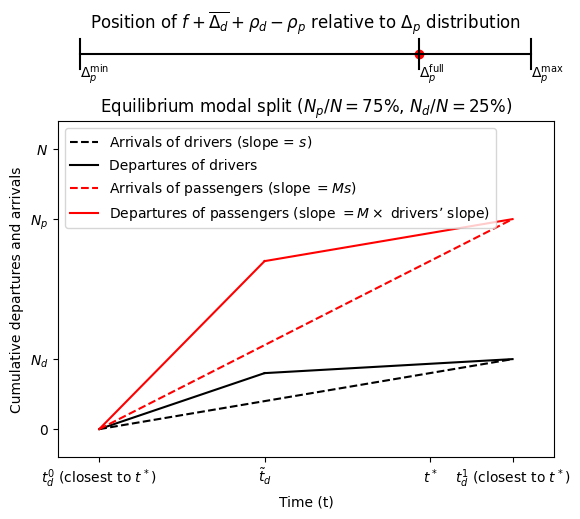
\includegraphics[width=\textwidth]{images/arrivals3.png}
        \caption{Full utilization of car capacity: equilibrium is unique for drivers and passengers}
    \end{center}
    \end{subfigure}

\caption{Departure and arrival rates of drivers and passengers for the three equilibrium regimes}
\label{fig_arrival_rates}

\end{center}
\end{figure}

\subsubsection{For $0 < \varphi < 1$}

Now, the three modes are allowed, so we can rewrite the previous definition:

\begin{definition}[Feasible modal split]
    A modal split $(N_s, N_d, N_p)$ is said to be feasible if $0 \leq N_p \leq M \times N_d$, $N_s \geq 0$ and $N_p + N_d + N_s = N$.    
\end{definition}

Similarly to the case $\varphi = 1$, it is clear that for some given $\rho _p$ and $\rho _d$, if there is an equilibrium, then it should lead to a feasible modal split as newly defined. If an equilibrium exist, solo-drivers and carpooling drivers would spread across time according to classical bottleneck time distribution (as defined in Equations \ref{eq_rs}, \ref{eq_ts}, \ref{eq_rd} and \ref{eq_td}). Passengers, if any, and as long as the car capacity is not reach, will never queue at the carpooling station while having no unique time-distribution. If the car capacity is reached, then, either it is possible to find a passenger that is indifferent between driving and carpooling as a passenger while all commuters with lower passenger inconvenience costs are passenger, in which case there is a unique equilibrium with a unique time distribution for passengers, othewise there is no equilibrium.

Then, the cost function for a commuter with a passenger inconvenience cost $\Delta _p$ is:

\begin{equation}
    \left\{
    \begin{array}{l}
        c_s(N_s) = \frac{\delta N_s}{(1-\varphi )s} + f\\
        c_d(N_d) = \frac{\delta N_d}{\varphi s} + f + \overline{\Delta _d} + \rho _d\\
        c_p(N_d, \Delta _p) = \frac{\delta N_d}{\varphi s} + \Delta _p + \rho _p
    \end{array} 
    \right.
\end{equation}

The conditions for having an equilibrium are:
\begin{itemize}
    \item If everybody drives solo ($N_s = N$, $N_d = 0$ and $N_p = 0$):
        \begin{equation}
            \label{eq_equilibrium_cond_start}
            c_d(0) \geq c_s(N) \leq c_p(0, \Delta _p)\quad \forall \Delta_p\in [\Delta_p^{\text{min}}, \Delta_p^{\text{max}}]
        \end{equation}
    
    \item If everybody drives on the \acrshort{rl} ($N_s = 0$, $N_d = N$ and $N_p = 0$):
        \begin{equation}
            c_s(0) \geq c_d (N) \leq c_p(N, \Delta _p^{\text{min}})
        \end{equation}

    \item If everybody carpools and the car capacity is reached ($N_s = 0$, $N_d = N\times \frac{1}{M+1}$ and $N_p = N\times \frac{M}{M+1}$):
        \begin{equation}
            \label{eq_equilibrium_Ns0_Nd_carfull}
            c_s(0) \geq c_d \left(\frac{N}{M+1}\right) = c_p\left(\frac{N}{M+1}, \Delta _p^{\text{full}}\right)
        \end{equation}

        Having $c_d \left(\frac{N}{M+1}\right) > c_p\left(\frac{N}{M+1}, \Delta _p^{\text{full}}\right)$ would lead to no equilibrium.

        
    \item If everybody carpools and the car capacity is not reached ($N_s = 0$, $\frac{N}{M+1} < N_d < N$ and $N_p = N - N_d$):
        \begin{equation}
            c_s(0) \geq c_d (N_d) = c_p\left(N_d, F^{-1} \left( \frac{N - N_d}{N} \right)\right)
        \end{equation}

    \item If some people drive solo and some share their seats, but without passengers ($0 < N_s < N$, $N_d = N - N_s$ and $N_p = 0$):
        \begin{equation}
            c_s(N_s) = c_d (N - N_s) \leq c_p(N - N_s, \Delta _p^{\text{min}})
        \end{equation}

    \item If some people drive, some other carpool, and the car capacity is reached ($0 < N_s < N$, $N_d = \frac{N-N_s}{M+1}$, and $N_p = (N-N_s)\times \frac{M}{M+1}$):
        \begin{equation}
        \label{eq_equilibrium_Ns_Nd_carfull}
            c_s(N_s) =  c_d \left( \frac{N-N_s}{M+1} \right) = c_p \left( \frac{N-N_s}{M+1}, F^{-1} \left( \frac{N-N_s}{N}\times \frac{M}{M+1} \right) \right)
        \end{equation}

        Having $c_d \left( \frac{N-N_s}{M+1} \right) > c_p \left( \frac{N-N_s}{M+1}, F^{-1} \left( \frac{N-N_s}{N}\times \frac{M}{M+1} \right) \right)$ would lead to no equilibrium.

    \item If some people drive, some other carpool, and the car capacity is not reached ($0 < N_s < N$, $\frac{N - N_s}{M+1} < N_d < N - N_s$, and $N_p = N - N_s - N_d$):
        \begin{equation}
            \label{eq_equilibrium_cond_finish}
            c_s(N_s) = c_d ( N_d ) = c_p\left(N - N_s - N_p, F^{-1}\left( \frac{N - N_s - N_p}{N} \right) \right)
        \end{equation}
\end{itemize}

Equations \ref{eq_equilibrium_cond_start} --- \ref{eq_equilibrium_cond_finish} might seem complicated to analyze. The nice proposition below will however help in making further manipulations handy.

\begin{prop}
\label{prop_feasible_modal_splits_and_fare_policies}
    \begin{itemize}
        \item For any given fare policy $(\rho _p,\rho _d)$:
        \begin{itemize}
            \item If
            \begin{equation*}
                \left\{
                \begin{array}{l}
                    \rho _d \leq - \frac{\delta}{\varphi s}\times \frac{N}{M+1} - \overline{\Delta _d}\\
                    \rho _p - \rho _d < f + \overline{\Delta _d} - \Delta _p^{\text{full}}
                \end{array}
                \right.
            \end{equation*}or
            \begin{equation*}
                \left\{
                \begin{array}{l}
                    -\frac{\delta}{\varphi s}\times \frac{N}{M+1} - \overline{\Delta _d} < \rho _d < \frac{\delta N}{(1-\varphi ) s} - \overline{\Delta _d}\\
                    \rho _p - \rho _d < f + \overline{\Delta _d} - F^{-1}\left( \frac{M}{(M+1)N} \times \left( N - \frac{\rho_d + \frac{\delta}{\varphi s}\times \frac{N}{M+1} + \overline{\Delta _d}}{\frac{\delta}{s}\times \left( \frac{1}{1-\varphi} + \frac{1}{\varphi (M+1)} \right)} \right)\right)
                \end{array}
                \right.
        \end{equation*}there is no equilibrium.
        
            \item Else, there exists a unique modal split that is an equilibrium. If the unique modal split is such that $0 < N_p < MN_d$, then the departure rate of passengers is non-unique. Otherwise, $N_p = 0$ or $N_p = MN_d$ and the departure rate of passengers is uniquely determined.

        \end{itemize}
        
        \item For any given feasible modal split, there exists a (non-necessary unique) fare policy $(\rho _p, \rho _d)$ such that the given modal split is the unique feasible modal split that is an equilibrium resulting from that fare policy. If the targeted feasible modal split either has $N_p = 0$ or $N_p = MN_d$, the departure rate of passengers is uniquely determined, otherwise it is not.
    \end{itemize}
\end{prop}

\begin{proof}
    The proof is structured as follows: for the first part of the proposition, we will first prove the uniqueness of the resulting feasible equilibrium (assuming existence) and then prove the existence for some fare policies and nonexistence for others; then will come the proof of the second part of the proposition.

    \item \paragraph{Proof that there is a unique feasible split for any fare policy}
    \item \subparagraph{Uniqueness}
    We first notice that, if $(N_s, N_d, N_p)$ is an equilibrium (regardless of feasibility), then $(N_p, N_d)$ must be an element of $\left\{ (N_d, N_p(N_d)) \quad \forall N_d\in\mathbb{R} \right\}$ where $N_p(N_d) := \min (M\times N_d, N \times F(f + \overline{\Delta _d} + \rho _d - \rho _p))$\footnotemark. Since this function is increasing and continuous, the function $N_d \longrightarrow N_d + N_p(N_d)$ is continuous and strictly increasing. There is thus at most one solution to the equation $N_d + N_p(N_d) = N$. Therefore, if $N_s = 0$, there is at most one feasible modal split that is an equilibrium.
    
    Similarly, if $0 < N_s < N$, then $N_d$ is also uniquely defined and can be written as $N_d (N_s) := \frac{\varphi}{1-\varphi}N_s - (\overline{\Delta _d} - \rho _d)\frac{\varphi s}{\delta}$ which is increasing and continuous. The function $N_s \longrightarrow N_s + N_d(N_s) + N_p(N_d(N_s))$ is strictly increasing and continuous. Therefore, there is at most one feasible modal split that is an equilibrium with $0 < N_s < N$.

    And of course, if $N_s = N$, there is at most one feasible modal split that is an equilibrium.
    
    \footnotetext{Here, $F$ is actually continued beyond $\Delta _p^{\text{min}}$ and $\Delta _p^{\text{max}}$ by setting $F(\Delta _p < \Delta _p^{\text{min}}) = 0$ and $F(\Delta _p > \Delta _p^{\text{max}}) = 1$} 

    To finish the proof of uniqueness, assume there exist two feasible modal splits that are equilibrium. We denote them $(N_s^0, N_d^0, N_p^0)$ and $(N_s^1, N_d^1, N_p^1)$. Due to the facts above, we are reduced to proving the assumption is absurd in each of the three following cases (or their symmetric):
    \begin{itemize}
        \item $N_s^0 = 0$ (1) and $N_s^1= N$ (2). Then, (1) implies $\frac{\delta N_d^0}{\varphi s} + \overline{\Delta _d} + \rho _d \leq 0$, and (2) implies $\overline{\Delta _d} + \rho _d \geq \frac{\delta N}{(1-\varphi)s}$. These two implications together imply that $\frac{\delta N_d^0}{\varphi s} + \frac{\delta N}{(1-\varphi)s} \leq 0$ which is impossible.

        \item $N_s^0 = 0$ (1) and $0 < N_s^1 < N$ (2). Then, (1) implies $\frac{\delta N_d^0}{\varphi s} + \overline{\Delta _d} + \rho _d \leq 0$, and (2) implies $\frac{\delta N_d^1}{\varphi s} + \overline{\Delta _d} + \rho _d = \frac{N_s^1}{(1-\varphi)s}$. These two together imply that $N_d^1 > N_d^0$, which in turn implies that $N_d^1 + N_p^1 > N_d^0 + N_p^0 = N$ which is impossible.
        \item $0 < N_s^0 < N$ (1) and $N_s^1 = N$ (2). Then, (1) implies $\frac{\delta N_d^0}{\varphi s} + \overline{\Delta _d} + \rho _d = \frac{N_s^0}{(1-\varphi)s}$, and (2) implies $\overline{\Delta _d} + \rho _d \geq \frac{\delta N}{(1-\varphi)s}$. These two together imply that $\frac{\delta N_s^0}{(1-\varphi)s} - \frac{\delta N_d^0}{\varphi s} \geq \frac{\delta N}{(1-\varphi)s}$ which is impossible.
    \end{itemize}

    We are now certain that if there is a feasible modal split that is an equilibrium, then this modal split is necessarily unique. It remains to prove under which conditions such an equilibrium actually exists.

    \item \subparagraph{Existence}

    To prove the existence we first prove that whatever the fare policy $(\rho_p, \rho_d) \in \mathbb{R}^2$, there exists a ``slack equilibrium''. A ``slack equilibrium'' is an equilibrium as determined by Equations \ref{eq_equilibrium_cond_start} --- \ref{eq_equilibrium_cond_finish} with two slight modification in the conditions. In Equations \ref{eq_equilibrium_Ns0_Nd_carfull} and \ref{eq_equilibrium_Ns_Nd_carfull}, the equality of costs between carpooling drivers and passengers becomes an inequality authorizing drivers cost to be higher than the highest carpooling cost. More specifically, Equation \ref{eq_equilibrium_Ns0_Nd_carfull} becomes
    \begin{equation}
    \label{eq_equilibrium_Ns0_Nd_carfull_slack}
        c_s(0) \geq c_d \left(\frac{N}{M+1}\right) \geq c_p\left(\frac{N}{M+1}, \Delta _p^{\text{full}}\right)
    \end{equation}
    and Equation \ref{eq_equilibrium_Ns_Nd_carfull} becomes
    \begin{equation}
    \label{eq_equilibrium_Ns_Nd_carfull_slack}
        c_s(N_s) =  c_d \left( \frac{N-N_s}{M+1} \right) \geq c_p \left( \frac{N-N_s}{M+1}, F^{-1} \left( \frac{N-N_s}{N}\times \frac{M}{M+1} \right) \right)
    \end{equation}
    
    Let $(\rho_p, \rho_d)$ be a fare policy, we define $c_{\text{min}} = \min (c_s(0), c_d(0)) = \min (f, f + \overline{\Delta _d} + \rho _d)$. Noticing that $c_s$ and $c_d$ are injective on $[c_s(0), +\infty[$ and $[c_d(0), +\infty[$ respectively, we also define the following two functions:
    
    \begin{equation}
        N_s(c):= c\in [c_{\text{min}}, +\infty[ \longrightarrow \left\{
        \begin{array}{lr}
            0 & \text{if } c \in [c_{\text{min}}, c_s(0)[\\
            c_s^{-1}(c) & \text{if } c \geq c_s(0)
        \end{array}
        \right.
    \end{equation}

    \begin{equation}
        N_d(c):= c\in [c_{\text{min}}, +\infty[ \longrightarrow \left\{
        \begin{array}{lr}
            0 & \text{if } c \in [c_{\text{min}}, c_d(0)[\\
            c_d^{-1}(c) & \text{if } c \geq c_d(0)
        \end{array}
        \right.
    \end{equation}

    And then, we define this other function:

    \begin{equation}
        c_p^{N_s, N_d}(N_s, N_d):= (N_s, N_d) \in \mathbb{R} _{+}^2 \longrightarrow \left[ N_p \in [0, M\times N_d] \longrightarrow c_p\left( N_d, F^{-1}\left(\frac{N_p}{N_s + N_d + N_p} \right) \right) \right]
    \end{equation}

    We can see that for all $(N_s, N_d) \in \mathbb{R} _{+}^2$, $c_p^{N_s, N_d}(N_s, N_d)$ is continuous strictly increasing in $N_p$, and therefore invertible. Using this fact, we construct two last intermediate functions:

    \begin{equation}
        N_p(c):= c\in [c_{\text{min}}, +\infty[ \longrightarrow
        \left\{
        \begin{array}{lr}
            0 & \text{if } c < c_p^{N_s, N_d} (N_s(c), N_d(c))(0)\\
            M\times N_d(c) & \text{if } c > c_p^{N_s, N_d} (N_s(c), N_d(c))(M\times N_d(c))\\
            c_p^{N_s, N_d} (N_s(c), N_d(c)) ^{-1} (c) & \text{else}
        \end{array}
        \right.
    \end{equation}

    \begin{equation}
        N(c):= c\in [c_{\text{min}}, +\infty[ \longrightarrow N_s(c) + N_d(c) + N_p(c)
    \end{equation}

    Finally, we note that $N_s(c)$, $N_d(c)$ and $N_p(c)$ are three continuous functions, and thus is $N(c)$\footnote{This is the point of the demonstration I am the less confident in. Even though I am personally very confident in that point I have had some difficulties in writing this formally. I am sure you could help with that}. Since $N(c_{\text{min}}) = 0$ and $\lim_{c\rightarrow +\infty} N(c) = +\infty$, there is at least one $c\in [c_{\text{min}}, +\infty[$ such that $N(c) = N$. By construction, the triplet $(N_s, N_d, N_p)$ thereby obtained is a feasible modal split satisfying one of the ``slack equilibrium'' conditions.

    We also note that the proof of uniqueness above also works for ``slack equilibria''. Therefore, the triplet is unique.
    
    To understand when this unique ``slack equilibrium'' is not an equilibrium, it remains to find under which conditions on the fare policy, the triplet thereby obtained either satisfies Equation \ref{eq_equilibrium_Ns0_Nd_carfull_slack} but not \ref{eq_equilibrium_Ns0_Nd_carfull}, or satisfies Equation \ref{eq_equilibrium_Ns_Nd_carfull_slack} but not \ref{eq_equilibrium_Ns_Nd_carfull}.

    \begin{itemize}
        \item In the first case (\ref{eq_equilibrium_Ns0_Nd_carfull_slack} but not \ref{eq_equilibrium_Ns0_Nd_carfull}), this is equivalent to
        \begin{equation}
            c_s(0) \geq c_d \left(\frac{N}{M+1}\right) > c_p\left(\frac{N}{M+1}, \Delta _p^{\text{full}}\right)
        \end{equation}which is equivalent to
        \begin{equation}
            \left\{
            \begin{array}{l}
                \rho _d \leq - \frac{\delta}{\varphi s}\times \frac{N}{M+1} - \overline{\Delta _d}\\
                \rho _p - \rho _d < f + \overline{\Delta _d} - \Delta _p^{\text{full}}
            \end{array}
            \right.
        \end{equation}

        \item In the second case (\ref{eq_equilibrium_Ns_Nd_carfull_slack} but not \ref{eq_equilibrium_Ns_Nd_carfull}), this is equivalent to 
        \begin{equation}
            c_s(N_s) =  c_d \left( \frac{N-N_s}{M+1} \right) > c_p \left( \frac{N-N_s}{M+1}, F^{-1} \left( \frac{M(N-N_s)}{N(M+1)} \right) \right)
        \end{equation}which is equivalent to
        \begin{equation}
            \left\{
            \begin{array}{l}
                \rho _d = \frac{\delta N_s}{(1- \varphi ) s} - \frac{\delta}{\varphi s}\times \frac{N-N_s}{M+1} - \overline{\Delta _d}\\
                \rho _p - \rho _d < f + \overline{\Delta _d} - F^{-1} \left( \frac{N-N_s}{N}\times \frac{M}{M+1} \right)
            \end{array}
            \right.
        \end{equation}

        In the context of $0 < N_s < N$, this implies

        \begin{equation}
            \left\{
            \begin{array}{l}
                -\frac{\delta}{\varphi s}\times \frac{N}{M+1} - \overline{\Delta _d} < \rho _d < \frac{\delta N}{(1-\varphi ) s} - \overline{\Delta _d}\\
                \rho _p - \rho _d < f + \overline{\Delta _d} - F^{-1}\left( \frac{M}{(M+1)N} \times \left( N - \frac{\rho_d + \frac{\delta}{\varphi s}\times \frac{N}{M+1} + \overline{\Delta _d}}{\frac{\delta}{s}\times \left( \frac{1}{1-\varphi} + \frac{1}{\varphi (M+1)} \right)} \right)\right)
            \end{array}
            \right.
        \end{equation}

        In the context of equilibrium, and using the uniqueness of the ``slack equilibrium'' above, we easily find that the last implication is actually an equivalence.
    \end{itemize}
    
    We finally find the conditions of the proposition for the existence of an equilibrium. This finishes the proof of the first part of the proposition.


    \item \paragraph{Proof that a feasible modal split always has a fare policy from which it could result as the unique equilibrium}
    
    Let $(N_s, N_d, N_p)$ be a feasible modal split.

    \begin{itemize}
        \item If $N_s = 0$, then we set $\rho _d \leq -\frac{\delta N_d}{\varphi s} - \overline{\Delta _d}$. As for $\rho _p$:
        \begin{itemize}
            \item If $N_d = N$, then we set $\rho _p \geq f + \rho _d + \overline{\Delta _d} - \Delta _p^{\text{min}}$.
            \item If $N_d = \frac{N}{M+1}$, then we set $\rho _p = f + \rho _d + \overline{\Delta _d} - \Delta _p^{\text{full}}$.
            \item Else, $\frac{N}{M+1} < N_d < N$, and we set $\rho _p = f + \rho _d + \overline{\Delta _d} - F^{-1}\left(\frac{N _p}{N} \right)$.
        \end{itemize}
        \item If, $N_s = N$, then we set $\rho _d \geq \frac{\delta N}{(1-\varphi)s} - \Delta _p$ and $\rho _p$ arbitrarily.
        \item Else, $0 < N_s < N$, and we set $\rho _d = \frac{\delta N_s}{(1-\varphi)s} - \frac{\delta N_d}{\varphi s} - \overline{\Delta _d}$. As for $\rho _p$:
        \begin{itemize}
            \item If $N_d = N - N_s$, then we set $\rho _p \geq f + \rho_d + \overline{\Delta _d} - \Delta _p ^{\text{min}}$.
            \item If $N_d = \frac{N - N_s}{M+1}$, then we set $\rho _p = f + \rho _d + \overline{\Delta _d} - F^{-1}\left( \frac{N - N_s}{N} \times \frac{M}{M+1} \right)$. This is one of the two only cases where the fare policy is uniquely defined.
            \item Else, $\frac{N - N_s}{M+1} < N_d < N - N_s$, and we set $\rho _p = f + \rho _d + \overline{\Delta _d} - F^{-1}\left(\frac{N _p}{N} \right)$. This is the second of the two only cases where the fare policy is uniquely defined.
        \end{itemize}
    \end{itemize}

    It is clear that the feasible modal split is an equilibrium with the fare policy defined above. Thanks to the first part of the proposition, it is also the only possible equilibrium that could result from that fare policy. This concludes the proof.
    

\end{proof}

This proposition is of great help for the remaining of the paper. We want indeed to compute the most desirable feasible modal splits. The fact that these modal splits will always be deterministically achievable by setting an appropriate fare policy (which has no impact on social cost functions) makes the optimization problems much simpler.

To better visualize how these equilibria behave, Figure \ref{fig_equilibrium_phase_diagram_trapezoidal_dist} provides a phase diagram of the different types of equilibria in a $(\rho_d, \rho_p)$ space. The equation of each line is written in Appendix \ref{appendix_equation_of_phase_diagram}.

\begin{figure}
    \centering
    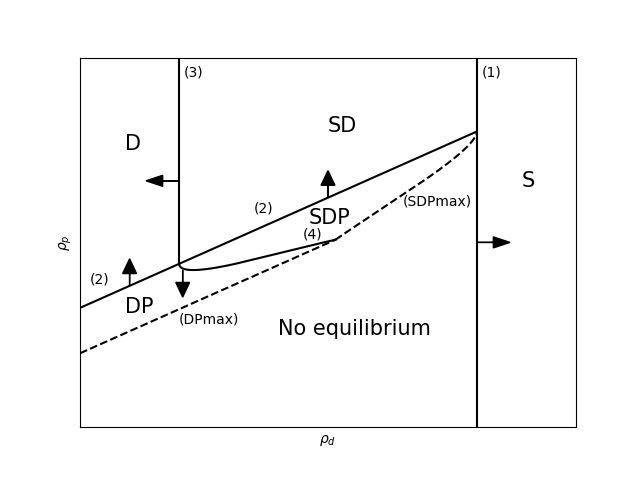
\includegraphics[trim=0cm 0cm 0cm 0cm, clip, width=0.5\linewidth]{images/equilibrium_phase_diagram_trapezoidal_dist.png}
    \caption{Phase diagram of equilibria in the fare policy space}
    \label{fig_equilibrium_phase_diagram_trapezoidal_dist}
\end{figure}
% could be great to see letters with meaning (s for solo, sd for solo and cp drivers…)

In this diagram, the values of $\overline{\Delta _d}$, $\Delta_p^{\text{min}}$, $\Delta _p^{\text{full}}$, $f$, $N$, $\varphi$ and $\delta$ only change the relative position of the line intersections without changing their relative positions, nor the slope of lines (1) and (3) (vertical) or lines (2) and (6) (slope of 1). However changing the function $F$ changes the shape of lines (4) and (5), but without changing their relative position to other lines. Especially, line (4) can not have a slope higher than 1, and line (5) must be increasing. For this specific example of diagram, a trapezoidal distribution was used, but with uniform distribution for example, lines (4) and (5) would become straight lines.

Dashed lines are equilibrium reduced to lines ((5) and (6)). They correspond to equilibrium where the capacity of cars is fully utilized and the departure rates of passengers is unique. Increasing $\rho _d$ or reducing $\rho_p$, even slightly, would make the model fall into the no-equilibrium area (area F)

The arrows on solid lines indicate to which area a line belongs to form an equilibrium space. Thus: \begin{itemize}
    \item Area A and line (1) define the fare policies for which everybody drives solo.
    \item Area B and the part of line (2) under it without its ends define the fare policies for which some people drive solo and some other share their seats on the reserved lane, but nobody carpools as a passenger.
    \item Area C, the part of line (2) under it, line (3) and the intersection of these two lines define the fare policies for which everyone offer their seats, but nobody is willing to be passenger.
    \item Area D and line (4) without it ends define the fare policies for which nobody drives solo, some people offer their seats, some other are passengers, but there are still some empty seats in some cars.
    \item Line (5) without its ends defines the fare policies for which some drive solo, some people offer their seats and the capacity of their car is fully used by passengers.
    \item Line (6) including its intersection with lines (4) and (5) define the fare policies for which nobody drives solo and the capacity of the cars are fully utilized.
    \item Area E defines the fare policies for which there is a mixture of the three modes without reaching the capacity of carpooling vehicles.
    \item And area F defines the fare policies from which no equilibrium could result.
\end{itemize}

\begin{remark}
    One can note that by navigating within area E and its contours, it is possible to obtain all feasible modal splits, and to obtain them only once. There is therefore a bijection between this closed subset of fare policies and the set of feasible modal splits. The second part of Proposition \ref{prop_feasible_modal_splits_and_fare_policies} could hence be rewritten as follows: ``For any given feasible modal split, there exists a unique fare policy in area E and its contour such that the given modal split is the unique feasible modal split that is an equilibrium resulting from that fare policy […]''
\end{remark}

\section{Draft}

As of here, I am not trying to write things in the clearest way, but simply to show the Maths so that they are not forgotten.

\subsection{Optimizing SC for fixed $\varphi = 1$}

The Lagrangian is

\begin{multline}
    \mathcal{L} = \frac{\delta}{s} (N_d^2 + N_d N_p) + N_d(\overline{\Delta_d} + f + E) + N\int_{\Delta_p^{\text{min}}}^{F^{-1}\left( \frac{N_p}{N} \right)} \Delta_p F'(\Delta_p)d\Delta_p\\
    - \lambda (N-N_d-N_p)\\
    -\mu_p(N_p - \alpha_p^2) - \mu_d(N_d - \alpha _d^2) - \mu_v(MN_d - N_p - \alpha _v^2)
\end{multline}

We write $\Delta_p^{\text{switch}} = F^{-1}\left( \frac{N_p}{N} \right)$. Deriving the Lagrangian gives:
\begin{eqnarray}
\label{eqnarray_varphi1_partialNd}
\frac{\partial \mathcal{L}}{\partial N_d} &=& \frac{\delta}{s} (2N_d + N_p) + \overline{\Delta_d} + f + E + \lambda - \mu_d - M\mu_v = 0\\
\label{eqnarray_varphi1_partialNp}
\frac{\partial \mathcal{L}}{\partial N_p} &=& \frac{\delta N_d}{s} + \Delta_p^{\text{switch}} + \lambda - \mu_p + \mu_v = 0\\
\frac{\partial \mathcal{L}}{\partial \lambda} &=& N - N_d - N_p = 0\\
\frac{\partial \mathcal{L}}{\partial \mu_d} &=& \alpha_d^2 - N_d = 0\\
\frac{\partial \mathcal{L}}{\partial \mu_p} &=& \alpha_p^2 - N_p = 0\\
\frac{\partial \mathcal{L}}{\partial \mu_v} &=& \alpha_v^2 - (MN_d - N_p) = 0
\end{eqnarray}

\begin{remark}
    Writing $N_p = N - N_d$ and deriving twice the objective function, we easily get a positive Hessian, meaning that the optimum is global and unique.
\end{remark}

It is impossible to have more than one active constraints in the three inequalities. It is also impossible not to have drivers. Therefore, we are left with the following three cases:

\begin{enumerate}
    \item \label{enum_item_no_passenger} $\mu_p > 0$, $\mu_d = 0$, $\mu_v = 0$;
    \item \label{enum_item_full_capacity} $\mu_p = 0$, $\mu_d = 0$, $\mu_v > 0$;
    \item \label{enum_item_interior} $\mu_p = \mu_d = \mu_v = 0$
\end{enumerate}

\paragraph{Case \ref{enum_item_no_passenger}} Equation \ref{eqnarray_varphi1_partialNd} and \ref{eqnarray_varphi1_partialNp} with conditions together give: $N_p = 0$, $N_d = N$, and $0 < \mu_p = \Delta_p^{\text{min}} - E - f - \overline{\Delta_d} - \frac{\delta N}{s}$. We could also calculate the value of $\lambda$ but we do not really care about it here.

\paragraph{Case \ref{enum_item_full_capacity}} Equation \ref{eqnarray_varphi1_partialNd} and \ref{eqnarray_varphi1_partialNp} with conditions together give: $N_p = \frac{MN}{M+1}$, $N_d = \frac{N}{M-1}$, and $0 < (M+1)\mu_v = \frac{\delta N}{s} + \overline{\Delta_d} + f + E - \Delta _p^{\text{full}}$.

\paragraph{Case \ref{enum_item_interior}} Equation \ref{eqnarray_varphi1_partialNd} and \ref{eqnarray_varphi1_partialNp} with conditions together give $\Delta_p^{\text{min}} < \Delta_p^{\text{switch}} = \frac{\delta N}{s} + \overline{\Delta_d} + f + E <\Delta_p^{\text{full}}$ which has only one solution.

\begin{remark}
    Interpreting these results is fairly straightforward. In case \ref{enum_item_no_passenger}, it should be the case that any commuter switching from driver to passenger when everyone drives raises social cost. By doing so, such a marginal switcher would reduce his congestion externality imposed to others by $\frac{\delta N}{s}$. At the same time he would enjoy a congestion relief for himself as a driver of $\frac{\delta N}{s}$, but incur the same congestion cost as a passenger being in the car of another driver. He would save the price of fuel $f$ and the inconvenience cost of drivers $\overline{\Delta_d}$. At the same time, the environment (and the economy depending from it) would enjoy a smaller externality of $E$. However, the new passenger would incur the inconvenience cost of being passenger, namely $\Delta _p$. Since this is true for all drivers, this is true in particular for the commuter with $\Delta_p = \Delta_p^{\text{min}}$, which gives the provided inequality.

    Similarly in case \ref{enum_item_interior}. It is clear that for any $N_p$, the best allocation is to have the $N_p$ commuters with the smallest $\Delta_p$ to be passengers (which is hopefully what happens in the considered equilibria). Then, the one at the frontier between the two modes should have the same contribution to social cost whatever the mode she chooses. As a driver, she generates the congestion externality of $\frac{\delta N_d}{s}$ for drivers and $\frac{\delta N_p}{s}$ for passengers, the environmental externality of $E$, and a personal cost (fares not included) of $f + \overline{\Delta_d} + \frac{\delta N_d}{s}$. As a passenger, he would not cause any externality but still incur a congestion cost of $\frac{\delta N_d}{s}$ in addition to $\Delta_p^{\text{switch}}$. This finally gives the provided first order condition of optimality.

    As for case \ref{enum_item_full_capacity}, a mixture of the two previous reasonings applies.
\end{remark}


\subsection{Optimizing SC for fixed $0 < \varphi < 1$}

This is where things get complicated. Now, the Lagrangian is:

\begin{multline}
    \mathcal{L} = \frac{\delta}{s}\left( \frac{N_s^2}{1-\varphi} + \frac{N_d^2 + N_d N_p}{\varphi}\right) + (N_d + N_s)(f+E) + N_d \overline{\Delta_d} + N \int_{\Delta_p^{\text{min}}}^{F^{-1}\left( \frac{N_p}{N} \right)} \Delta_p F'(\Delta_p) d \Delta_p\\
    -\lambda(N - N_s - N_d - N_p)\\
    -\mu_s(N_s - \alpha_s^2) -\mu_d(N_d - \alpha_d^2) -\mu_p(N_p - \alpha_p^2) -\mu_v(MN_d - N_p - \alpha_v^2)
\end{multline}

We write $\Delta_p^{\text{switch}} = F^{-1}\left( \frac{N_p}{N} \right)$. Deriving the Lagrangian gives:
\begin{eqnarray}
\label{eqnarray_varphi1_partialNs2}
\frac{\partial \mathcal{L}}{\partial N_s} &=& \frac{2\delta N_s}{(1-\varphi)s} + f + E + \lambda - \mu_s = 0\\
\label{eqnarray_varphi1_partialNd2}
\frac{\partial \mathcal{L}}{\partial N_d} &=& \frac{\delta}{\varphi s} (2N_d + N_p) + \overline{\Delta_d} + f + E + \lambda - \mu_d - M\mu_v = 0\\
\label{eqnarray_varphi1_partialNp2}
\frac{\partial \mathcal{L}}{\partial N_p} &=& \frac{\delta N_d}{\varphi s} + \Delta_p^{\text{switch}} + \lambda - \mu_p + \mu_v = 0\\
\frac{\partial \mathcal{L}}{\partial \lambda} &=& N - N_d - N_p = 0\\
\frac{\partial \mathcal{L}}{\partial \mu_s} &=& \alpha_s^2 - N_s = 0\\
\frac{\partial \mathcal{L}}{\partial \mu_d} &=& \alpha_d^2 - N_d = 0\\
\frac{\partial \mathcal{L}}{\partial \mu_p} &=& \alpha_p^2 - N_p = 0\\
\frac{\partial \mathcal{L}}{\partial \mu_v} &=& \alpha_v^2 - (MN_d - N_p) = 0
\end{eqnarray}

\begin{remark}
    Replacing $N_s$ by $N - N_p - N_d$, we get the following objective function:

    \begin{equation*}
        SC = \frac{\delta}{s}\left( \frac{(N - N_p - N_d)^2}{1-\varphi} + \frac{N_d^2 + N_d N_p}{\varphi}\right) + (N - N_p)(f+E) + N_d \overline{\Delta_d} + N \int_{\Delta_p^{\text{min}}}^{F^{-1}\left( \frac{N_p}{N} \right)} \Delta_p F'(\Delta_p) d \Delta_p
    \end{equation*}

    Then, calculating the gradient, we get:
    \begin{equation*}
    \nabla_f (N_d, N_p) = 
    \begin{pmatrix}
        \frac{\delta}{s} \left( \frac{-2(N-N_p-N_d)}{1-\varphi} + \frac{2N_d}{\varphi} + \frac{N_p}{\varphi} \right) + \overline{\Delta_d}\\
        \frac{\delta}{s} \left( \frac{-2(N-N_p-N_d)}{1-\varphi} + \frac{N_d}{\varphi} \right) -f-E + F^{-1}\left( \frac{N_p}{N} \right)
    \end{pmatrix}
    \end{equation*}

    And then, the Hessian is:

    \begin{equation*}
        H_f(N_d, N_p) =
        \begin{pmatrix}
            \frac{2\delta}{s}\left(\frac{1}{1-\varphi} + \frac{1}{\varphi}\right) &
            \frac{\delta}{s}\left(\frac{2}{1-\varphi} + \frac{1}{\varphi}\right)\\
            \frac{\delta}{s}\left(\frac{2}{1-\varphi} + \frac{1}{\varphi}\right) &
            \frac{2\delta}{(1-\varphi )s} + \frac{1}{NF'\left(F^{-1}\left( \frac{N_p}{N} \right)\right)}
        \end{pmatrix}
    \end{equation*}

    which is strictly positive definite. Since we are solving a convex function on a convex space, the minimum is necessary global and unique.
\end{remark}

To understand which combinations of $\mu_i > 0$ should be explored, we exhaust the possibilities in Table \ref{table_cases_for_fixed_interior_phi_optim}.

\begin{table}
    \centering
    \begin{tabular}{|c|c|c|c|m{8cm}|}
        \hline
        $\mu_s > 0$ & $\mu_d > 0$ & $\mu_p > 0$ & $\mu_v > 0$ & Conclusion\\
        \hline
        \hline
        False & False & False & False & To explore (should lead to interior solution)\\
        \hline
        False & False & False & True & To explore (should lead to both lanes being used with exhaustion of seat capacity on reserved lane)\\
        \hline
        False & False & True & False & To explore (should lead to both lanes being used without passengers)\\
        \hline
        False & False & True & True & To explore (should lead to $N_s = N$)\\
        \hline
        False & True & False & False & To explore (should lead to $N_s = N$)\\
        \hline
        False & True & False & True & To explore (should lead to $N_s = N$)\\
        \hline
        False & True & True & False & To explore (should lead to $N_s = N$)\\
        \hline
        False & True & True & True & To explore (should lead to $N_s = N$)\\
        \hline
        True & False & False & False & To explore (should lead to $N_s = 0$ and interior solution for the reserved lane)\\
        \hline
        True & False & False & True & To explore (should lead to $N_s = 0$ and car capacity being exhausted)\\
        \hline
        True & False & True & False & To explore (should lead to $N_d = N$)\\
        \hline
        True & False & True & True & Impossible (would lead to $N_s = N_d = N_p = 0$)\\
        \hline
        True & True & False & False & Impossible (would lead to $N_s = N_d = N_p = 0$)\\
        \hline
        True & True & False & True & Impossible (would lead to $N_s = N_d = N_p = 0$)\\
        \hline
        True & True & True & False & Impossible (would lead to $N_s = N_d = N_p = 0$)\\
        \hline
        True & True & True & True & Impossible (would lead to $N_s = N_d = N_p = 0$)\\
        \hline
    \end{tabular}
    \caption{Exhaustion of combinations of $\mu_i > 0$}
    \label{table_cases_for_fixed_interior_phi_optim}
\end{table}



Now we explore what has to be explored:
\paragraph{Case $\mu_d = \mu_v = 0$, $\mu_s > 0$ and $\mu_p >0$:} We have $N_d = N$. We find the two intuitive conditions: $\overline{\Delta _d} < -\frac{2\delta N}{\varphi s}$ and $\Delta _p^{\text{min}} > \frac{\delta N}{\varphi s} + \overline{\Delta_d} + f + E$. While the intuition for the second inequality has already been detailed, the one for the first inequality is also straightforward: by choosing to drive solo on the non reserved lane, the driver reduces her congestion cost by $\frac{\delta N}{\varphi s}$, and her congestion externality by the same amount. This reduction should be higher than what is gained socially when she offers her seats ($-\overline{\Delta_d}$).

\paragraph{Case $\mu_d = \mu_p = 0$, $\mu_s > 0$ and $\mu_v >0$:} We have $N_d = \frac{N}{M+1}$ and $N_p = N - N_d$. This time, we get the three following conditions: $\Delta_p^{\text{full}} < \frac{\delta N}{\varphi s} + f + E + \overline{\Delta_d}$, $\Delta_p^{\text{full}} + \frac{\delta N}{\varphi s (M+1)} < f+E$, and $M(f+E) > M\Delta _p^{\text{full}} + \frac{2 \delta N}{\varphi s}  + \overline{\Delta_d}$. The intuition for the last inequality is subtle. Take a marginal user with passenger inconvenience cost of $\Delta_p^{\text{full}}$ and divide it in $M+1$ sub-users. Provide them with to choices. Either drive solo, or have $M$ sub-users who are passengers and $1$ sub-user who is driver. In the first case, they would create a social cost $(M+1)(f+E)$. In the second case, the driver would create a social cost for fuel and environment of $f+E$, but also cause a congestion externality of $\frac{\delta N}{\varphi s}$, incur the same congestion cost as well as a driver inconvenience cost of $\overline{\Delta_d}$, and the $M$ passengers will face an inconvenience cost of $M\Delta_p^{\text{full}}$. The second option should be preferred.

\paragraph{Case $\mu_d = \mu_p = \mu_v = 0$ and $\mu_s >0$:} We have $N_p = N\times F^{-1} \left( \frac{\delta N}{\varphi s} + f + E + \overline{\Delta_d}\right)$ and $N_d = N - N_p$. Here we get $\Delta_p^{\text{min}} \leq \Delta_p^{\text{switch}} = \frac{\delta N}{\varphi s} + f + E + \overline{\Delta_d} < \Delta_p^{\text{full}}$, and $f+E > \frac{\delta N_d}{\varphi s} + \Delta_p^{\text{switch}}$. While the writing of the last inequality is intuitive, we rewrite it $\frac{\delta N}{\varphi s} \left( 2 - F^{-1} \left( \frac{\delta N}{\varphi s} + f + E + \overline{\Delta_d} \right) \right) + \overline{\Delta_d} < 0$ to make it independent of other variables.

\paragraph{Case $\mu_s = 0$, $\mu_d > 0$, $\mu_p > 0$ and $\mu_v >0$:} We have $N_s = N$. We find the two condition: $\overline{\Delta_d}>\frac{2\delta N}{(1 - \varphi ) s}$ and $M\Delta_p^{\text{min}} + \overline{\Delta_d} > (M+1)\frac{2\delta N}{(1 - \varphi ) s} + Mf + ME$. Once again, this has a very intuitive interpretation: offering seats without getting anyone is pointless. From this stand point, the only hope is to form a carpool with all the seats occupied. But even then, it is better for $M+1$ marginal sub-users to drive solo than to organize a carpool.

\paragraph{Case $\mu_s = \mu_v = 0$, $\mu_d > 0$ and $\mu_p > 0$:} We have $N_s = N$. We get again the two conditions of the previous case: $\overline{\Delta_d} > \frac{2\delta N}{(1 - \varphi ) s}$ and $M\Delta_p^{\text{min}} + \overline{\Delta_d} > (M+1)\frac{2\delta N}{(1 - \varphi ) s} + Mf + ME$. Moreover, we get the intuitive additional condition: $\Delta_p^{\text{min}} > \frac{2\delta N}{(1 - \varphi ) s} + f + E$.

\paragraph{Case $\mu_s = \mu_p = 0$, $\mu_d > 0$ and $\mu_v > 0$:} We have $N_s = N$. Here, we find four conditions: $\Delta_p^{\text{min}} < \frac{2\delta N}{(1 - \varphi ) s} + f + E$, $\Delta_p^{\text{min}} < \overline{\Delta_d} + f + E$ and again the inequalities $\overline{\Delta_d} > \frac{2\delta N}{(1 - \varphi ) s}$ and $M\Delta_p^{\text{min}} + \overline{\Delta_d} > (M+1)\frac{2\delta N}{(1 - \varphi ) s} + Mf + ME$.

\paragraph{Case $\mu_s = \mu_p = \mu_v = 0$ and $\mu_d > 0$:} We have $N_s = N$. Here, we find: $\Delta_p^{\text{min}} = \frac{2\delta N}{(1 - \varphi ) s} + f + E$ (carpooling as a passenger and driving solo are the same from a social cost standpoint), $\Delta_p^{\text{min}} < \overline{\Delta_d} + f + E$ (even when carpooling, it would be better not to drive), and the classical two inequalities, namely $\overline{\Delta_d} > \frac{2\delta N}{(1 - \varphi ) s}$ and $M\Delta_p^{\text{min}} + \overline{\Delta_d} > (M+1)\frac{2\delta N}{(1 - \varphi ) s} + Mf + ME$. However, the equality with the two first inequalities leads to impossibility. This case is therefore not feasible.

\paragraph{Case $\mu_s = \mu_d = 0$, $\mu_p > 0$ and $\mu_v > 0$:} We have $N_s = N$. Here, we find the two classical inequalities, namely $\overline{\Delta_d} > \frac{2\delta N}{s}$ and $M\Delta_p^{\text{min}} + \overline{\Delta_d} > (M+1)\frac{2\delta N}{s} + Mf + ME$. We note that this case might prove to be impossible in some cases.



\paragraph{Case $\mu_s = \mu_d = \mu_v = 0$ and $\mu_p > 0$:} We get $0 \leq N_s = N(1-\varphi)\left( 1 + \varphi \frac{\Delta_d}{2\delta N /s} \right) \leq N$ and $N_d = N - N_s$. And $\Delta_p^{\text{min}} > \frac{\delta N_d}{\varphi s} + f +E + \overline{\Delta_d}$. To make the last inequality dependent only on setting variables, we can rewrite it in a less intuitive way as $\Delta_p^{\text{min}} + \frac{\delta N}{s}\times \frac{1-\varphi}{\varphi}\times \left( 1 + \varphi \frac{\Delta_d}{2\delta N /s} \right) > \frac{\delta N}{\varphi s} + f +E + \overline{\Delta_d}$.

\paragraph{Case $\mu_s = \mu_d = \mu_p = 0$ and $\mu_v > 0$:} $N_s$ is the unique solution of $Mf + ME + (M+1)\frac{2\delta N_s}{(1-\varphi)s} = \frac{2\delta (N-N_s)}{\varphi s} + MF^{-1}\left( \frac{(N-N_s)\frac{M}{M+1}}{N} \right) + \overline{\Delta _d}$ between $0$ and $N$ (left hand side is continuous strictly increasing and right hand side is continuous strictly decreasing with $N_s$, so if there is a solution, it is unique). This gives two conditions: $M(f+E) \leq \frac{2\delta N}{\varphi s}$ and $M\Delta_p^{\text{min}} \leq M(f+E) + \frac{2\delta N}{(1-\varphi )s}$. Then $N_d =\frac{N-N_s}{M+1}$ and $N_p = N - N_s - N_p$. We also find the condition $\Delta_p^{\text{switch}} < \overline{\Delta_d} + f + E + \frac{\delta (N - N_s)}{\varphi s}$ where $\Delta_p^{\text{switch}} = F^{-1}\left( \frac{(N-N_s)\frac{M}{M+1}}{N} \right)$

\paragraph{Case $\mu_s = \mu_d = \mu_p = \mu_v = 0$:} Je n’arrive pas à trouver ma solution intérieure… Ni à synthétiser les résultats à la fin…

\clearpage
\part{Appendices}
\appendix

\section{Equations of Figure \ref{fig_equilibrium_phase_diagram_trapezoidal_dist}}
\label{appendix_equation_of_phase_diagram}

In this appendix, we write down the equations of the lines shown in Figure \ref{fig_equilibrium_phase_diagram_trapezoidal_dist}.

\begin{itemize}
    \item Line (1):
    \begin{equation*}
        \rho_d = \frac{\delta N}{(1-\varphi)s}
    \end{equation*}

    \item Line (2):
    \begin{equation*}
        \left\{
        \begin{array}{l}
            \rho_d < \frac{\delta N}{(1 - \varphi)s} - \overline{\Delta _d}\\
            \rho_p = \rho_d + f + \overline{\Delta_d} - \Delta_p^{\text{min}}
        \end{array}
        \right.
    \end{equation*}

    \item Line (3):
    \begin{equation*}
        \left\{
        \begin{array}{l}
            \rho_d = \frac{-\delta N}{\varphi s} - \overline{\Delta_d}\\
            \rho_p > \rho_d + f + \overline{\Delta_d} - \Delta_p^{\text{min}}
        \end{array}
        \right.
    \end{equation*}

    \item Line (4):
    \begin{equation*}
        \left\{
        \begin{array}{l}
            \rho_d = \rho_d(N_d) = -\frac{\delta N_d}{\varphi s} - \overline{\Delta_d}\\
            \rho_p = \rho_p(N_d) = \rho_d(N_d) + f + \overline{\Delta_d} - F^{-1}\left( \frac{N - N_d}{N} \right)
        \end{array}
        \right. \qquad \forall N_d \in \left]\frac{N}{M+1}, N\right[
    \end{equation*}

    \item Line (5):
    \begin{equation*}
        \left\{
        \begin{array}{l}
            \rho_d = \rho_d (N_s) = \frac{\delta N_s}{(1-\varphi)s} - \frac{\delta}{\varphi s} \times \frac{N - N_s}{M+1} - \overline{\Delta_d}\\
            \rho_p = \rho_p(N_s) = \rho_d(N_s) + f + \overline{\Delta_d} - F^{-1} \left( \frac{N - N_s}{N} \times \frac{M}{M+1} \right)
        \end{array}
        \right.
        \qquad \forall N_s \in \left]0, N\right[
    \end{equation*}

    \item Line (6):
    \begin{equation*}
        \left\{
        \begin{array}{l}
            \rho_d \leq - \frac{\delta}{\varphi s} \times \frac{N}{M+1} - \overline{\Delta_d}\\
            \rho_p = \rho_d + f + \overline{\Delta_d} - \Delta_p^{\text{full}}             
        \end{array}
        \right.
    \end{equation*}
    
\end{itemize}


% Parler du projet TRAPEZE et déclaration de conflit d’intérêt.
% parler de l’instabilité quand Delta_d varie avec la possibilité d’avoir un passager.


\section{restarting all calculations for it was s*** till then}
%TODO we might have to change this title later on ;)

Fixed $\varphi \in ]0, 1[$

Fixed $\Delta_p$.

Fixed $\Delta_d$


The Lagrangian becomes:

\begin{multline}
\label{eq_lagrangian_linear}
    \mathcal{L} = \frac{\delta}{s} \left( \frac{(N - N_d - N_p)^2}{1 - \varphi} + \frac{N_d (N_d + N_p)}{\varphi} \right) + (N - N_p)(f+E) + N_d \Delta_d + N_p \Delta_p\\
    -\mu_s(N - N_p - N_d) - \mu_d N_d - \mu_p N_p - \mu_v (M N_d - N_p)
\end{multline}

Deriving the Lagrangian, we get:

\begin{eqnarray}
    \frac{\partial \mathcal{L}}{\partial N_d} & = & \frac{\delta}{s} \left( -\frac{2(N - N_d - N_p)}{1 - \varphi} + \frac{2N_d + N_p}{\varphi} \right) + \Delta_d + \mu_s - \mu_d - M \mu_v = 0\\
    \frac{\partial \mathcal{L}}{\partial N_p} & = & \frac{\delta}{s} \left( -\frac{2(N - N_d - N_p)}{1 - \varphi} + \frac{N_d}{\varphi} \right) -f-E + \Delta_p + \mu_s - \mu_p + \mu_v = 0\\
    \frac{\partial \mathcal{L}}{\partial \mu_s} & = & N_p + N_d - N = 0\\
    \frac{\partial \mathcal{L}}{\partial \mu_d} & = & -N_d = 0\\
    \frac{\partial \mathcal{L}}{\partial \mu_p} & = & -N_p = 0\\
    \frac{\partial \mathcal{L}}{\partial \mu_v} & = & N_p - MN_d = 0\\
\end{eqnarray}

We first check for convexity of our objective function (first line of equation \ref{eq_lagrangian_linear}.

The gradient is:

\begin{equation}
    \nabla_{SC} (N_d, N_p) = \begin{pmatrix}
        \frac{\delta}{s} \left( -\frac{2(N - N_d - N_p)}{1 - \varphi} + \frac{2N_d + N_p}{\varphi} \right) + \Delta_d\\
        \frac{\delta}{s} \left( -\frac{2(N - N_d - N_p)}{1 - \varphi} + \frac{N_d}{\varphi} \right) -f-E + \Delta_p
    \end{pmatrix}
\end{equation}

The Hessian is:

\begin{equation}
    H_{SC} (N_d, N_p) = \begin{pmatrix}
        \frac{2\delta}{s} \left( \frac{1}{1 - \varphi} + \frac{1}{\varphi} \right) & \frac{\delta}{s} \left( \frac{2}{1 - \varphi} + \frac{1}{\varphi} \right)\\
        \frac{\delta}{s} \left( \frac{2}{1 - \varphi}  + \frac{1}{\varphi} \right) & \frac{2\delta}{(1 - \varphi) s}
    \end{pmatrix}
\end{equation}.

The determinant is $-\left(\frac{\delta}{\varphi s}\right)^2$. Which is negative. One of the two eigen values is therefore negative and the other is positive, meaning that there is no interior solutions, since every cancellation of the gradient should happen at saddle point of $SC$. As a consequence, we are looking only for corner solutions and their conditions. Then we should compare the finite set of corner solutions whose conditions to choose the best one.

Then we find some solutions that are in the python of my other laptop. I skip them to go straight to the final result:

\begin{description}
    \item [Case a:]\label{dis_case_a} $N_d = N$, $N_s = N_p = 0$. Conditions are:
    \begin{itemize}
        \item $\Delta_d + \frac{2\delta N}{\varphi s} < 0$
        \item $\Delta_p > E + f + \Delta_d + \frac{\delta N}{\varphi s}$
    \end{itemize}
    \item [Case b:]\label{dis_case_b} $N_d = \frac{N}{M + 1}$, $N_p = \frac{NM}{M+1}$ and $N_s = 0$. Conditions are:
    \begin{itemize}
        \item $M(f+E) > M\Delta_p + \Delta_d + \frac{2\delta N}{\varphi s}$
        \item $E + f + \Delta_d + \frac{\delta N}{\varphi s} > \Delta_p$
    \end{itemize}
    \item [Case c:]\label{dis_case_c} $N_s = 0$, and all $(N_d, N_p)$, complying with the following conditions:
    \begin{itemize}
        \item $N_d \geq 0$
        \item $N_p \geq 0$
        \item $N_p \leq MN_d$
        \item $N_p = N - N_d$
        \item $\Delta_d + \frac{2\delta N}{\varphi s} < \frac{\delta N_p}{\varphi s}$
        \item $f+E+\Delta_d + \frac{\delta N}{\varphi s} = \Delta_p$
    \end{itemize}

    \item [Case defgh:]\label{dis_case_defgh} $N_s = N$, $N_d = N_p = 0$. Conditions are:
    \begin{itemize}
        \item $\Delta_d > \frac{2\delta N}{(1 - \varphi )s}$
        \item $M \Delta_p + \Delta_d > M(E + f) + (M+1) \frac{2\delta N}{(1 - \varphi )s}$
    \end{itemize} % TODO, this should be decomposed actually

    \item [Case i:] \label{dis_case_i} $N_p = 0$, $N_d = \varphi \left( N - \Delta_d \middle/ \frac{2\delta}{(1- \varphi) s} \right)$ and $N_s = N - N_d$. Conditions are
    \begin{itemize}
        \item $-\frac{2\delta N}{\varphi s} \leq \Delta_d \leq \frac{2\delta N}{(1-\varphi ) s}$
        \item $2\Delta_p > 2(E + f) + \Delta_d(1 + \varphi) + \frac{2 \delta N}{s}$
    \end{itemize}

    \item [Case j:] \label{dis_case_j} $N_d = \frac{N \varphi}{M\varphi + 1} + s\varphi (1 - \varphi) \frac{M(E + f - \Delta_p) - \Delta_d}{2\delta (M + 1)(M\varphi + 1)}$, $N_p = M N_d$ and $N_s = N - N_d(M + 1)$. Conditions are:
    \begin{itemize}
        \item $-\frac{2\delta N}{\varphi s} \leq \Delta_d + M(\Delta_p - E - f) \leq \frac{2\delta N (M + 1)}{(1-\varphi)s}$
        \item $\frac{2\delta N(M+1)}{s} + \Delta_d(2M\varphi + \varphi + 1) + (E + f - \Delta_p)(M\varphi + M + 2) > 0$
    \end{itemize}
\end{description}

Then we can check that the conditions cover the full space.

TODO INSERT PICTURE HERE BUT ON MY OTHER LAPTOP.

To do so, we check that for all values of $\Delta_d$, there is always at least one case whose candititions are satisfied for all values of $\Delta_p$.

\begin{description}
    \item[Case $\Delta_d > \frac{2\delta N}{(1-\varphi) s}$:]
    \begin{description}
        \item[If $M(\Delta_p - E - f) + \Delta_d > (M+1) \frac{2\delta N}{1-\varphi)s}$:] This is case \emph{defgh}.
        \item[If $(M+1)\frac{2\delta N}{(1-\varphi)s} \geq M(\Delta_p - E - f) + \Delta_d \geq -\frac{2\delta N}{\varphi s}$:] $\frac{2\delta N(M+1)}{s} + \Delta_d(2M\varphi + \varphi + 1) + (E + f - \Delta_p)(M\varphi + M + 2) \geq \frac{2\delta N(M+1)}{s} + \Delta_d(2M\varphi + \varphi + 1) + (\Delta_d - (M+1)\frac{2\delta N}{(1-\varphi)s})(M\varphi + M + 2)/M = \frac{2(M\varphi + 1)}{M}\times \frac{2\delta N}{s} \left( -1 + \frac{M+1}{1-\varphi} \right) > 0$. So conditions of case \emph{j} are satisfied.

        \item[If $M(\Delta_p - E - f) + \Delta_d +\frac{2\delta N}{\varphi s} < 0$:] We get $f + E - \Delta_p + \Delta_d + \frac{\Delta N}{\varphi s} > (M + 1) \Delta_d + \frac{(M+2)\delta N}{\varphi s} >0$. We recognize the conditions of case \emph{b}.
    \end{description}
    \item[Case $-\frac{\delta N(M+2)}{\varphi s(M+1)} < \Delta_d \leq \frac{2\delta N}{(1-\varphi)s}$:]
    \begin{description}
        \item[If $2\Delta_p > 2(E + f) + \Delta_d (1 + \varphi) + \frac{2\delta N}{(1 - \varphi )s}$:] Since $2 > \frac{M+2}{M+1}$, we have $\Delta_d \geq -\frac{2\delta N}{\varphi s}$. So we recognize the conditions of case \emph{i}.
        
        \item[If $2\Delta_p \leq 2(E + f) + \Delta_d (1 + \varphi) + \frac{2\delta N}{(1 - \varphi )s}$:] It is a bit more complicated.
        
        First, we note that at $\Delta_d = \frac{2\delta N}{(1-\varphi ) s}$, $2\Delta_p \leq 2(E + f) + \Delta_d (1 + \varphi) + \frac{2\delta N}{(1 - \varphi )s}$ leads to $\Delta_p - \Delta_d = E + f$. And therefore, under the two assumptions that $\Delta_d = \frac{2\delta N}{(1-\varphi ) s}$ and $2\Delta_p \leq 2(E + f) + \Delta_d (1 + \varphi) + \frac{2\delta N}{(1 - \varphi )s}$, we have that $\frac{2\delta N(M+1)}{s} + \Delta_d(2M\varphi + \varphi + 1) + (E + f - \Delta_p)(M\varphi + M + 2) = (M\varphi + M + 2)(E + f - \Delta_p + \Delta_d) = 0$. Then, using the facts that $\frac{M\varphi + M + 2}{1 + \varphi + 2M \varphi} > \frac{1 + \varphi}{2}$ ($M > M\varphi$ and $2 > 1 + \varphi$), we have that $\forall\Delta_d < \frac{2\delta N}{(1-\varphi) s}$, $2\Delta p \leq 2(E + f) + \Delta_d(1+\varphi) + \frac{2\delta N}{s}$ implies $\frac{2\delta N(M+1)}{s} + \Delta_d(2M\varphi + \varphi + 1) + (E + f - \Delta_p)(M\varphi + M + 2) > 0$.

        Then we notice that for $\Delta_d > -\frac{M+2}{M+1}\cdot\frac{\delta N}{\varphi s}$ and $M(f+E) > M\Delta_p + \Delta_d + \frac{2\delta N}{\varphi s}$, we also have $M(\Delta_p - f - E) < -\Delta_d - \frac{2\delta N}{\varphi s} < -\Delta_d + \Delta_d \frac{2(M+1)}{M+2} = \Delta_d \frac{M}{M+2} = M\Delta_d - \Delta_d \frac{M(M+1)}{M+2} < M(\Delta_d + \frac{\delta N}{\varphi s})$.

        Therefore, we end with the following case exhaustion for $-\frac{\delta N(M+2)}{\varphi s(M+1)} < \Delta_d \leq \frac{2\delta N}{(1-\varphi)s}$ and $2\Delta_p \leq 2(E + f) + \Delta_d (1 + \varphi) + \frac{2\delta N}{(1 - \varphi )s}$, as long as the two last inequalities are not equal together:
        \begin{itemize}
            \item If $-\frac{2\delta N}{\varphi s} \leq \Delta_d + M(\Delta_p - E - f)$, we are in case \emph{j}.
            \item Otherwise, we are in case \emph{b}.
        \end{itemize}

        The case where both equalities occur together still has to be solved. %TODO important.

    \end{description}    
    \item[Case $\Delta_d \leq-\frac{\delta N(M+2)}{\varphi s(M+1)}$:] This time, it is much simpler. We have three cases:
    \begin{description}
        \item[If $\Delta_p < E + f + \Delta_d + \frac{\delta N}{\varphi s}$:] Here, we find $M(f+E-\Delta_p) > -M \Delta_d - M\frac{\delta N}{\varphi s} = \Delta_d - (M+1)\Delta_d - M\frac{\delta N}{\varphi s}$. Using $-(M+1) \Delta_d \geq (M+2)\frac{\delta N}{\varphi s}$. We find $M(f+E - \Delta_p) > \Delta_d + \frac{2 \delta N}{\varphi s}$ and recognize the conditions of case \emph{b}.

        \item[If $\Delta_p = E + f+ \Delta_d + \frac{\delta N}{\varphi s}$:] For $\Delta_d < -\frac{M+2}{M+1}\cdot\frac{\delta N}{\varphi s}$, we easily get $\Delta_d + \frac{2\delta N}{\varphi s} < \frac{\delta N_p}{\varphi s}$, and recognize the conditions of case \emph{c}.

        \item[If $\Delta_p > E + f + \Delta_d + \frac{\delta N}{\varphi s}$:] Then, $\Delta_d \leq \frac{M+2}{M+1}\cdot\frac{\delta N}{\varphi s} < -\frac{\delta N}{\varphi s}$, and we recognize the conditions of case \emph{a}.
    \end{description}
\end{description}

    The point where $\Delta_p = E + f+ \Delta_d + \frac{\delta N}{\varphi s}$ and $\Delta_d = -\frac{M+2}{M+1}\cdot\frac{\delta N}{\varphi s}$ is still to be solved.
    %TODO

    The two points are actually not a problem since we could replace strict inequalities by loose inequalities.

    \subsection{Limit when $N \rightarrow 0$}

    We assume $\varphi$ can only take up values between $\varepsilon$ and $1 - \varepsilon$ (where $\varepsilon > 0$ is a small number).

    \begin{itemize}
        \item If $\Delta_d < 0$: \begin{itemize}
            \item If $\Delta_p > E + f + \Delta_d$. Then for $N\rightarrow 0$, case \emph{a} will be satisfied whatever the value of $\varphi$. Similarly, case \emph{b}, \emph{defgh} and \emph{i} will not be satisfied for all values of $N$ whatever the value of $\varphi$. The equality of case \emph{c} will also not be satisfied at some point. As for case \emph{j}. It could be satisfied only if $\Delta_d = M(E + f - \Delta_p)$. But the inequality $\frac{2\delta N(M+1)}{s} + \Delta_d(2M\varphi + \varphi + 1) + (E + f - \Delta_p)(M\varphi + M + 2) > 0$ would lead to $\Delta_d > 0$, which is contradictory. So only case \emph{a} could be satisfied for a sufficiently small $N$.

            \item If $\Delta_p \leq E + f + \Delta_d$. Then for $N\rightarrow 0$. It is not hard to see that for a small enough $N > 0$, cases \emph{a}, \emph{c}, \emph{defgh}, \emph{i} and \emph{j} cannot be satisfied. However, we easily obtain that $M(f + E) \geq \Delta_d + M\Delta_p - (M+1)\Delta_d > \Delta_d + M\Delta_p$, which shows that case \emph{b} will be satisfied for a sufficiently small $N$.
        \end{itemize}

        \item If $\Delta_d > 0$: \begin{itemize}
            \item If $\Delta_d + M\Delta_p > M(E+f)$. It is straightforward to see that cases \emph{a}, \emph{b}, \emph{c}, \emph{i} and \emph{j} cannot be satisfied, and that case \emph{defgh} is satisfied.
            \item If $\Delta_d + M\Delta_p < M(E+f)$. This time, it case \emph{b} that is the only feasible case for sufficiently small values of $N>0$
            \item If $\Delta_d + M\Delta_p = M(E+f)$ Then, only case \emph{j} can be satisfied for small $N$.
        \end{itemize}

        \item If $\Delta_d = 0$: \begin{itemize}
            \item If $\Delta_p > E + f$. It is straighforward to see that cases \emph{a}, \emph{b}, \emph{c}, \emph{defgh} and \emph{j} cannot be satisfied for small $N$, while case \emph{i} will be.
            \item If $\Delta_p < E + f$. It is case \emph{b} which the only one to be satisfied for small $N$.
            \item If $\Delta_p = E + f$, case \emph{j} is the only one that is satisfied for small enough values of $N$.
        \end{itemize}
    \end{itemize}

        Let us now choose the best value of $\varphi \in [\varepsilon, 1 - \varepsilon]$ for $N \rightarrow 0$.

        Since the case exhaustion above was true whatever the value of $\varphi \in [\varepsilon, 1 - \varepsilon]$, we can check the values of $SC$ for a varying $\varphi$ and a small enough $N$.

        \begin{description}
            \item[Case a:] $SC = \frac{\delta N^2}{\varphi s} + N (E + f + \Delta_d)$. And $\frac{\partial SC}{\partial \varphi} = -\frac{\delta N^2}{\varphi ^2 s} < 0$. Therefore, the best $SC$ is obtained for $\varphi = 1- \varepsilon$. Moreover, using $\Delta_d < 0$, we get for sufficiently small $N$, $\frac{\delta N^2}{s} + N(E + f + \Delta_d) < \frac{\delta N^2}{(1 - \varepsilon)s} + N (E + f + \Delta_d) < \frac{\delta N^2}{s} + N(E+ f)$. We also know that the best thing to do when $\varphi = 1$ is to have only drivers. Therefore, \textbf{the best thing to do is to reserve 100\% of the capacity and set $N_d = N$}.

            \item[Case b:] $SC = \frac{\delta N^{2}}{\varphi s (M+1)} + (E + f + \Delta_d + M \Delta_p)\frac{N}{M+1}$. And $\frac{\partial SC}{\partial \varphi} = -\frac{\delta N^2}{\varphi ^2 s (M+1)} < 0$. Therefore, the best $SC$ is obtained for $\varphi = 1- \varepsilon$. Moreover, using $M(f+ E - \Delta_p) > \Delta_d$, we get for sufficiently small $N$, $\frac{\delta N^2}{s(M+1)} + N(E + f + \Delta_d + M\Delta _p) < \frac{\delta N^2}{s(M+1)(1 - \varepsilon)} + N(E + f + \Delta_d + M\Delta _p) < \frac{\delta N^2}{s} + N(E+ f)$. We also know that the best thing to do when $\varphi = 1$ is to have as many passengers as could be fitted in cars. Therefore, \textbf{the best thing to do is to reserve 100\% of the capacity and set $N_d = \frac{N}{M+1}$ and $N_p = \frac{NM}{M+1}$}.

            \item[Case defgh:] $SC = \frac{\delta N^2}{(1- \varphi)s} + N(E + f)$. And $\frac{\partial SC}{\partial \varphi} = \frac{\delta N^2}{(1 - \varphi) ^2 s} > 0$. Therefore, the best $SC$ is obtained for $\varphi = \varepsilon$. Moreover, using both facts that $\frac{N_p}{N} \leq M\frac{N_d}{N}$ and $\Delta_d > M(E + f -\Delta_p)$, we get that for a sufficiently small $N$, for all $N_d \in \left[ \frac{N}{M+1}, N\right]$, $N\left[ \frac{\delta}{s} \left( N_d - \frac{N}{1 - \varepsilon} + \left( 1 - \frac{N_d}{N} \right) (\Delta_p - E - f) + \frac{N_d}{N}\Delta_d \right) \right] > 0$. Therefore, for a sufficiently small $N$, and for all $N_d \in \left[ \frac{N}{M+1}, N\right]$, $\frac{\delta N^2}{s} + N(E + f) < \frac{\delta N^2}{(1 - \varepsilon)s} + N(E + f) < \frac{\delta N_d N}{s} + \Delta _d\frac{N_d}{N} + \Delta_p \left(1 - \frac{N_d}{N} \right)$. Therefore, \textbf{the best thing to do is to keep 100\% of the capacity to solo-drivers}.

            \item[Case i:] Here, we use Sympy [ref] $\frac{\partial SC}{\partial \varphi} = \Delta_d \left( N + \left( \varphi - \frac{1}{2}\right) \frac{\Delta_d s}{2 \delta} \right)$. However, according to the case exhaustion above, case \emph{i}, as $N$ becomes small, conditions of case \emph{i} could be satisfied only if $\Delta_d = 0$. We hence have $\frac{\partial SC}{\partial \varphi} = 0$ and the value of $SC$ is insensitive to the value of $\varphi$. Using the fact that $\Delta_d = 0$, we get $\frac{\delta N^2}{s} + N(E + f + \Delta_d) = \frac{\delta N^2 (1 - \varphi)^2}{(1 - \varphi)s} + \frac{\delta N^2 \varphi^2}{\varphi s} + N(E + f) + \varphi N\Delta_d$. Also, since $\Delta_p > E + f$, we know that the best thing to do with $\varphi = 1$ is to set $N_d = N$. Therefore, \textbf{the best thing to do is to reserve whatever capacity we like, while respecting the modal split $N_s = (1-\varphi)s$ and $N_d = \varphi s$}.

            \item[Case j:] Again, we use Sympy [ref] to make the calculations. We find
            \begin{equation}
                \frac{\partial SC}{\partial \varphi} = \frac{1}{B}\left[ \frac{M A^2 s^2}{4} \times \varphi^2  + \frac{A^2 s^2}{2} \times \varphi - N^2 \delta ^2 M (M+ 1) + N\delta s A(M+1) -\frac{A^2 s^2}{4} \right]
            \end{equation} Where $A = \Delta_d + M(\Delta_p - E - f)$, and $B = \delta s (M+1)(M\varphi + 1)^2 >0$. From the case exhaustion above, we know that conditions of case \emph{j} can be satisfied for small $N$ only if $A = 0$. So we end up with $\frac{\partial SC}{\partial \varphi} = -\frac{N^2\delta M(M+1)}{B} < 0$. And therefore, the best value of $SC$ is obtained for $\varphi = 1 - \varepsilon$. Moreover, after some calculations using the fact that $\Delta_d + M\Delta_p = M(f + E)$, we find that $SC_{\varphi = 1 - \varepsilon} = \frac{\delta N^2}{(M\varphi + 1)s} + N(f+E)$. For $\varphi = 1$, using the fact that $\Delta_d \geq 0$, we easily get that the best is to maximize the number of passengers in cars, and $SC_{\varphi = 1} = \frac{\delta N^2}{(M + 1)s} + N(f+E)$. For $\varphi = 0$, $SC_{\varphi = 0} = \frac{\delta N^2}{s} + N(f+E)$. Since $SC_{\varphi = 1} < SC_{\varphi = 1-\varepsilon} < SC_{\varphi = 0}$, \textbf{the best thing to do is to reserve 100\% of the capacity while filling cars as much as possible}.
        \end{description}

    To summarize: we have the following decision tree for $N \rightarrow 0$:

    
    Question: $\Delta_d < 0$ or $\Delta_d + M\Delta_p \leq M(E+f)$?
    \begin{itemize}
        \item YES. Set $\varphi = 1$. Question: $\Delta_d \geq 0$ or $\Delta_p \leq E + f + \Delta_d$?
        \begin{itemize}
            \item YES. Set $N_d = \frac{N}{M + 1}$ and $N_p = \frac{MN}{M+1}$.
            \item NO. Set $N_d = N$ and $N_p = 0$.
        \end{itemize}
        \item NO. Question: $\Delta_d > 0$?
        \begin{itemize}
            \item YES. Set $\varphi = 0$ and $N_s = N$.
            \item NO. Set $\varphi \in [0, 1]$, $N_d = \varphi N$ and $N_s = (1-\varphi ) N$
        \end{itemize}
    \end{itemize}

    \subsection{Limit when $N \rightarrow +\infty$}

    Here it is simpler. We first see that for a big enough $N$. The only case that could be satisfied is case \emph{j}.

    Similarly, we quickly check that for $\varphi = 1$, the best is to maximize car filling rate.

    Hence, we have that $SC_{\varphi = 1} = \frac{\delta N^2}{(M+1)s} + o(N^2)$, $SC_{\varphi = 0} = \frac{\delta N^2}{s} + o(N^2)$, and $SC_{\varphi \in [\varepsilon, 1 - \varepsilon]} = \frac{\delta N^2}{s} \times \frac{1 + M\varphi + (1 - \varphi)}{(1 + M\varphi)^2} + o(N^2)$, where $o(N^2)$ describes any function $g(N)$ for which $g(N) / N^2 \rightarrow 0$ as $N \rightarrow +\infty$ . While it is obvious that for a high enough $N$, $SC_{\varphi = 1} < SC_{\varphi = 0}$. It is less straightforward to see that $SC_{\varphi = 1} < SC_{\varphi \in [\varepsilon, 1 - \varepsilon]}$. To see that, we check that $\frac{1 + M\varphi + (1 - \varphi)}{(1 + M\varphi)^2} - \frac{1}{M+ 1} = \frac{(1 -\varphi)((M+1)^2 - M^2(1 -\varphi)}{(1 + M\varphi)^2 (M+1)} > 0$.

    We can conclude that whatever the value of epsilon, there is a Value of $N$ for which it is best to reserve 100\% of the capacity while filling the cars as much as possible.

    PROBLEM, il n’y a pas d’équilibre avec $\Delta_p$ qui ne varie pas. Sauf si l’on distribue les droits de paiements…


    \section{And once again we start with a variable $\Delta_p$}

    \subsection{$\varphi = 1$}

    Equation of social cost is:

    \begin{equation}
        SC_{\varphi = 1} = \frac{\delta NN_d}{s} + N_d (f+E + \Delta_d) + N\int_{\Delta_p^{\text{min}}}^{F^{-1} \left( \frac{N - N_d}{N} \right)} \Delta_p F'(\Delta_p) d\Delta_p
    \end{equation}

    With $N_d \in \left[ \frac{N}{M+1}, 1 \right]$

    Differentiating according to $N_d$ gives

    \begin{equation}
        \frac{dSC_{\varphi = 1}}{dN_d} = \frac{\delta N}{s} + f + E + \Delta_d - F^{-1}\left( 1 - \frac{N_d}{N} \right)
    \end{equation}

    Clearly the second order conditions means that canceling this derivative leads to optimum. Therefore:

    \begin{itemize}
        \item If $\frac{\delta N}{s} + f + E + \Delta_d < \Delta_p^{\text{min}}$: solution is $N_d = N$, $N_p = 0$. Everybody drives solo. This is not very realistic since we could expect $\Delta_d$ to be ineffective.
        \item If $\frac{\delta N}{s} + f + E + \Delta_d > \Delta_p^{\text{full}}$: solution is $N_d = \frac{N}{M+1}$, $N_p = \frac{MN}{N+1}$, everybody carpools up to car capacity.
        \item Else, there exist a $\Delta_p^{switch} = \frac{\delta N}{s} + f + E + \Delta_d \in [\Delta_p^{\text{min}}, \Delta_p^{\text{full}}]$: solution is $N_p = NF(\Delta_p^{\text{switch}})$ and $N_d = N - N_p$. Carpooling exist but there are still some empty seats in cars.
    \end{itemize}
    
    \subsection{$\varphi = 0$}

    Here solution is much simpler. Nobody carpools by definition and social cost is always the same:

    \begin{equation}
        SC_{\varphi = 0} = \frac{\delta N^2}{s} + N (f+E)
    \end{equation}

    \subsection{$\varphi \in ]0, 1[$}

    Here it gets more complexe:

    Social Cost is:

    \begin{equation}
        \frac{\delta}{s} \left ( \frac{(N - N_d - N_p)^2}{1- \varphi} + \frac{N_d(N_d + N_p)}{\varphi} \right)
        + (N - N_p) (f+E)
        + N_d \Delta_d + N \int_{\Delta_p^{\text{min}}}^{F^{-1} \left ( \frac{N_p}{N} \right)} \Delta_p F'(\Delta_p) d\Delta_p
    \end{equation}.

    The gradient is:

    \begin{equation}
        \nabla_{SC} (N_d, N_p) = \begin{pmatrix}
            \frac{\delta}{s} \left( \frac{-2(N - N_d - N_p)}{1 - \varphi} + \frac{2 N_d + N_p}{\varphi} \right) + \Delta_d\\
            \frac{\delta}{s} \left( \frac{-2(N - N_d - N_p)}{1 - \varphi} + \frac{N_d}{\varphi} \right) -f - E + F^{-1} \left( \frac{N_p}{N} \right)
        \end{pmatrix}
    \end{equation}

    The Hessian is:

    \begin{equation}
        H_{SC}(N_d, N_p) = \begin{pmatrix}
            \frac{2 \delta}{s} \left( \frac{1}{1 - \varphi} + \frac{1}{\varphi} \right) & \frac{\delta}{s} \left( \frac{2}{1 - \varphi} + \frac{1}{\varphi} \right)\\
            \frac{\delta}{s} \left( \frac{2}{1 - \varphi} + \frac{1}{\varphi} \right) & \frac{2\delta}{(1- \varphi )s} + \frac{1}{NF'\left(F^{-1}\left(\frac{N_p}{N} \right)\right)}
        \end{pmatrix}
    \end{equation}

    Then, since the matrix is real symmetric, it has real eigenvalues.

    We calculate:

    \begin{multline}
        \left| H_{SC} - \lambda I \right| = \lambda^2\\
        -\lambda \left[ \frac{2\delta (1 + \varphi)}{\varphi (1 - \varphi ) s} + \frac{1}{NF'\left( F^{-1}\left( N_p/N \right) \right)} \right]\\
        - \left( \frac{\delta}{\varphi s}\right)^2 + \frac{2\delta}{\varphi (1 -\varphi) s N F'(F^{-1}(N_p / N))}
    \end{multline}

    Using classical $\frac{-b \pm \sqrt{b^2 - 4 ac}}{2a}$, it is easy to see that at least one eigen value is positive and the other could be either positive (for points where the slope of $F$ is small and $\varphi$ is close to $1$), or negative (for points where the slope of $F$ is big or $\varphi$ is close to $0$). It is therefore not sure whether there will be interior solutions or not.
    
    The Lagrangian Equation is 

    \begin{multline}
        \frac{\delta}{s} \left ( \frac{(N - N_d - N_p)^2}{1- \varphi} + \frac{N_d(N_d + N_p)}{\varphi} \right)
        + (N - N_p) (f+E)
        + N_d \Delta_d + N \int_{\Delta_p^{\text{min}}}^{F^{-1} \left ( \frac{N_p}{N} \right)} \Delta_p F'(\Delta_p) d\Delta_p\\
        -\mu_s(N - N_p - N_d) - \mu_d N_d - \mu_p N_p - \mu_v(MN_d - N_p)
    \end{multline}

    As always, all combinations of constraints being active or not are theoretically possible. However, after a closer inspection, some are not. Therefore, we only explore the feasible combinations.


    \subsubsection{Case a: $\mu_s > 0$ ($N_p + N_d = N$), $\mu_d = 0$ ($N_d \geq 0$), $\mu_p > 0$ ($N_p = 0$) and $\mu_v = 0$ ($N_p \leq MN_d$)}

    We find:

    \begin{itemize}
        \item $N_d = N$
        \item $N_p = 0$
        \item $N_s = 0$
        \item $\frac{2\delta N}{\varphi s} + \Delta_d < 0$ (from $\mu_s$). The intuition is simply that driving and sharing seats is more satisfying than going alone on an empty road.
        \item $\frac{\delta N}{\varphi s} + f + E + \Delta_d < \Delta_p^{\text{min}}$ (from $\mu_p$). The intuition is that being a passenger is very repulsive.
    \end{itemize}

    This case is not very realistic in the sense that if there is no passenger, then drivers may never really experience their negative $\Delta_d$.

    \subsubsection{Case b: $\mu_s > 0$ ($N_p + N_d = N$), $\mu_d = 0$ ($N_d \geq 0$), $\mu_p = 0$ ($N_p \geq 0$) and $\mu_v > 0$ ($N_p = MN_d$)}

    We find:

    \begin{itemize}
        \item $N_d = \frac{N}{M+1}$
        \item $N_p = \frac{MN}{M+1}$
        \item $N_s = 0$
        \item $\frac{\delta N}{\varphi s} + \Delta_d + f + E > \Delta_p^{\text{full}}$ (from $\mu_v$). The intuition is that, if it were possible, it would be better to have more drivers switch to passengers, but cars are already full…
        \item $\frac{2\delta N}{\varphi s} + \Delta_d + M\Delta_p^{\text{full}} < M(f + E)$ (from $\mu_s$). The intuition is that it is better to put $M+1$ marginal users as carpoolers (one being the driver of the $M$ others) than having (M+1) solo-drivers.
    \end{itemize}

    \subsubsection{Case c: $\mu_s > 0$ ($N_p + N_d = N$), $\mu_d = 0$ ($N_d \geq 0$), $\mu_p = 0$ ($N_p \geq 0$) and $\mu_v = 0$ ($N_p \leq MN_d$)}

    We find:

    \begin{itemize}
        \item $N_d = N - N_p$
        \item $N_p = NF\left( \frac{\delta N}{\varphi s} + \Delta_d + f + E \right)$
        \item $N_s = 0$
        \item $\Delta_p^{\text{min}}\leq \frac{\delta N}{\varphi s} + \Delta_d + f + E \leq \Delta_p^{\text{full}}$ (from $\mu_v$ and $\mu_p$ complementary constraints). The intuition is that without solo-drivers, an equilibrium is to be found about the number of drivers and passengers.
        \item $\frac{\delta N}{\varphi s} + \frac{\delta N_d}{\varphi s} + \Delta_d <0$ (from $\mu_s$). The intuition is that it is better to make a marginal user a carpooling driver than a solo-driver, where $\frac{\delta N}{\varphi s}$ is the congestion externality of being a carpooling driver, and $\frac{\delta N_d}{\varphi s}$ is the congestion cost incurred by the driver.
    \end{itemize}

    \subsubsection{Case d: $\mu_s = 0$ ($N_p + N_d \leq N$), $\mu_d > 0$ ($N_d = 0$), $\mu_p > 0$ ($N_p = 0$) and $\mu_v > 0$ ($N_p = MN_d$)}

    Here manipulation are slightly less straightforward for we find parametric equations in the conditions. An equivalent, but not parametric set of conditions is given below:

    \begin{itemize}
        \item $N_s = N$
        \item $N_p = 0$
        \item $N_d = 0$
        \item $\Delta_d > \frac{2\delta N }{(1 - \varphi)s}$
        \item $\Delta_d + M \Delta_p^{\text{min}} > M(f+ E) + \frac{2\delta N (M+1)}{(1 - \varphi) s}$
    \end{itemize}

    \subsubsection{Case e: $\mu_s = 0$ ($N_p + N_d \leq N$), $\mu_d > 0$ ($N_d = 0$), $\mu_p > 0$ ($N_p = 0$) and $\mu_v = 0$ ($N_p \leq MN_d$)}

    We find:

    \begin{itemize}
        \item $N_s = N$
        \item $N_p = 0$
        \item $N_d = 0$
        \item $\Delta_d > \frac{2\delta N }{(1 - \varphi)s}$ (from $\mu_d$)
        \item $\Delta_p^{\text{min}} > f+ E + \frac{2\delta N}{(1 - \varphi) s}$ (from $\mu_p$)
    \end{itemize}

    \subsubsection{Case f: $\mu_s = 0$ ($N_p + N_d \leq N$), $\mu_d > 0$ ($N_d = 0$), $\mu_p = 0$ ($N_p \geq 0$) and $\mu_v > 0$ ($N_p = MN_d$)}

    We find:

    \begin{itemize}
        \item $N_s = N$
        \item $N_p = 0$
        \item $N_d = 0$
        \item $\Delta_p^{\text{min}} < f+ E + \frac{2\delta N}{(1 - \varphi) s}$ (from $\mu_v$)
        \item $\Delta_d + M \Delta_p^{\text{min}} > M(f+ E) + \frac{2\delta N (M+1)}{(1 - \varphi) s}$ (from $\mu_d$)
    \end{itemize}


    \subsubsection{Case g: $\mu_s = 0$ ($N_p + N_d \leq N$), $\mu_d > 0$ ($N_d = 0$), $\mu_p = 0$ ($N_p \geq 0$) and $\mu_v = 0$ ($N_p \leq MN_d$)}

    We find:
    
    \begin{itemize}
        \item $N_s = N$
        \item $N_p = 0$
        \item $N_d = 0$
        \item $\Delta_p^{\text{min}} = f+ E + \frac{2\delta N}{(1 - \varphi) s}$
        \item $\Delta_d >\frac{2\delta N}{(1 - \varphi) s}$ (from $\mu_d$)
    \end{itemize}
    

    \subsubsection{Case h: $\mu_s = 0$ ($N_p + N_d \leq N$), $\mu_d = 0$ ($N_d \geq 0$), $\mu_p > 0$ ($N_p = 0$) and $\mu_v > 0$ ($N_p = MN_d$)}

    We find:

    \begin{itemize}
        \item $N_s = N$
        \item $N_p = 0$
        \item $N_d = 0$
        \item $\Delta_d >\frac{2\delta N}{(1 - \varphi) s}$ (from $\mu_v$)
        \item $\Delta_d + M \Delta_p^{\text{min}} > M(f+ E) + \frac{2\delta N (M+1)}{(1 - \varphi) s}$ (from $\mu_p$ and $\mu_v$)
    \end{itemize}

    \begin{remark}
        For all cases \emph{d-h}, conditions always imply that:

        \begin{itemize}
        \item $\Delta_d >\frac{2\delta N}{(1 - \varphi) s}$
        \item and $\Delta_d + M \Delta_p^{\text{min}} > M(f+ E) + \frac{2\delta N (M+1)}{(1 - \varphi) s}$
        \end{itemize}
        Therefore, we refer to this case as case \emph{defgh}.
    \end{remark}

    

    \subsubsection{Case i: $\mu_s = 0$ ($N_p + N_d \leq N$), $\mu_d = 0$ ($N_d \geq 0$), $\mu_p > 0$ ($N_p = 0$) and $\mu_v = 0$ ($N_p \leq MN_d$)}

    We find:

    \begin{itemize}
        \item $N_d = \varphi \left( N - \frac{\Delta_d}{\left. 2\delta \middle/ (1-\varphi)s  \right.} \right)$
        \item $N_p = 0$
        \item $N_s = N - N_d$
        \item $-\frac{2\delta N}{\varphi s} \leq \Delta_d \leq \frac{2\delta N}{(1-\varphi) s}$
        \item $2\Delta_p^{\text{min}} > (1 + \varphi)\Delta_d + 2(f + E + \frac{\delta N}{s})$
    \end{itemize}
    

    \subsubsection{Case j: $\mu_s = 0$ ($N_p + N_d \leq N$), $\mu_d = 0$ ($N_d \geq 0$), $\mu_p = 0$ ($N_p \geq 0$) and $\mu_v > 0$ ($N_p = MN_d$)}

    We find:

    \begin{itemize}
        \item $N_d$ is the unique solution of
        \begin{equation}A = \frac{2\delta (M+1)}{s} \left[ \frac{-N}{1-\varphi} + \frac{1 + M\varphi}{\varphi(1-\varphi)}N_d \right] + \Delta_d + M \left[ F^{-1}\left( \frac{MN_d}{N} \right) - f - E \right] = 0
        \label{eq_compstatcond_casej}
        \end{equation}
        \item $N_p = MN_d$
        \item $N_s = N - (M+1) N_d$
        \item $M\Delta_p^{\text{min}} -\frac{2\delta N(M+1)}{(1-\varphi)s} \leq M(f+E) - \Delta_d \leq M\Delta_p^{\text{full}} + \frac{2\delta N}{\varphi s}$
        \item $\frac{\delta}{s} \left[ \frac{-2(N - (M+1)N_d)}{1 -\varphi} + \frac{(M+2)N_d}{\varphi} \right] + \Delta_d > 0$ (from $\mu_v$)
    \end{itemize}

    \subsubsection{Case k: $\mu_s = 0$ ($N_p + N_d \leq N$), $\mu_d = 0$ ($N_d \geq 0$), $\mu_p = 0$ ($N_p \geq 0$) and $\mu_v = 0$ ($N_p \leq MN_d$)}

    Finally, for this case, we find:

    \begin{itemize}
        \item $N_p$ should be a solution of $B = -\frac{\delta N}{s} + \frac{\delta N_p}{(1-\varphi)s} \left( 2 - \frac{(1+\varphi)^2}{2\varphi} \right) - \frac{\Delta_d (1+\varphi)}{2} - f - E + F^{-1}\left( \frac{N_p}{N} \right) = 0$
        \item $N_d = N\varphi - N_p\frac{1+\varphi}{2} - \frac{\Delta_d (1-\varphi)\varphi s}{2\delta}$
        \item $0 \leq N_p \leq \frac{MN}{M+1}$
        \item $\frac{N_p}{M} \leq N_d$
        \item $N_d \leq N - N_p$
        \item $|H_{SC}(N_d, N_p)| \geq 0$ (and higher order conditions if it is $0$)
    \end{itemize}

    Here, it may be that many $(N_d, N_p)$ are solutions, as well as none.

    \subsection{$\varphi$ is exogenous and $N \rightarrow 0$}

    As seen in case exhaustion below, it is independent of $\varphi$.
    
    \begin{itemize}
        \item Case a: $N_d / N = 1$, $N_p / N = 0$, $N_s / N = 0$, $\Delta_d < 0$ and $f + E + \Delta_d < \Delta_p^{\text{min}}$.
        \item Case b: $N_d / N = \frac{1}{M + 1}$, $N_p / N = \frac{M}{M + 1}$, $N_s / N= 0$, $\Delta_d + f + E \geq \Delta_p^{\text{full}}$ and $\Delta_d + M\Delta_p^{\text{full}} < M(f+ E)$.
        \item Case c: $N_p / N \rightarrow F(\Delta_d + f + E)$, $N_s / N = 0$, $N_d / N \rightarrow 1 - N_p / N$, $\Delta_p^{\text{min}} \leq \Delta_d + f + E < \Delta_p^{\text{full}}$ and $\Delta_d < 0$.
        \item Case defgh: $N_s / N = 1$, $N_p / N = 0$, $N_d / N = 0$, $\Delta_d > 0$ and $\Delta_d + M\Delta_p^{\text{min}} > M(f + E)$.
        \item Case i: $N_d / N = \varphi$, $N_p / N = 0$, $N_s / N = 1 - N_d / N$, $\Delta_d = 0$ and $\Delta_p^{\text{min}} > f + E$
        \item Case j: $N_d / N \rightarrow \frac{1}{M} F\left( f + E - \frac{\Delta_d}{M} \right)$, $N_p / N \rightarrow F\left( f + E - \frac{\Delta_d}{M} \right)$, $N_s / N \rightarrow 1 - \frac{M+ 1}{M}F\left( f + E - \frac{\Delta_d}{M} \right)$, $M\Delta_p^{\text{min}} \leq M(f + E) - \Delta_d \leq M\Delta_p^{\text{full}}$ and 1. $\Delta_d > 0$ if $\frac{-2(N - (M + 1)N_d)}{1 - \varphi} + \frac{(M+ 2)N_d}{\varphi} < 0$ (which is equivalent to $F(f + E) < \frac{2M\varphi}{2 + M + M\varphi}$, or 2. $\Delta_d \geq 0$ otherwise. 
        \item Case k: $\Delta_d = 0$ (due to $N_d = N\varphi - N_p\frac{1 + \varphi}{2} - \frac{\Delta_d(1 - \varphi)\varphi s}{2\delta}$. $N_p / N \rightarrow F(f + E)$, $N_d / N \rightarrow \varphi - \frac{1 + \varphi}{2} F(f + E)$, $N_s /N \rightarrow (1 - \varphi)\left( 1 - \frac{1}{2}F(f + E)\right)$, $0\leq N_p / N \leq \frac{M}{M + 1}$ (which is equivalent to $\Delta_p^{\text{min}} \leq f + E \leq \Delta_p^{\text{full}}$, $\frac{N_p / N}{M} \leq N_d / N$ (which is equivalent to $F(f + E)\leq \frac{2M\varphi}{2 + M + M\varphi}$, $N_d / N + N_p / N \leq 1$ (which is equivalent to $F(f + E) \leq 2$ which is always true), the Hessian condition is always true as it goes to infinity with $N \rightarrow 0$.
    \end{itemize}

    \subsection{$\varphi$ is exogenous and $N \rightarrow +\infty$}

    The only case available is case j. $N_d / N \rightarrow \frac{\varphi}{1 + M\varphi}$, $N_p / N \rightarrow \frac{M\varphi}{1 + M\varphi}$ and $N_s / N \rightarrow \frac{1 - \varphi}{1 + M\varphi}$.

    

    %todo exemplify

    \subsection{Endogenize for $\varphi \in [\varepsilon, 1 - \varepsilon]$ ($\varepsilon$ is small)}

    Additional to the optimal conditions seen previously, we add some other conditions deriving from a differentiation of $SC$ relative to $\varphi$.

    \subsubsection{Case a:}
    $N_d = N$, $N_p = N_s = 0$
    
    \[
    SC = \frac{\delta N^2}{\varphi s} + N(f + E + \Delta_d)
    \]

    \[
    \frac{d SC}{d \varphi} = -\frac{\delta N^2}{\varphi^2 s} < 0
    \]
    
    Therefore, $\varphi = 1 - \varepsilon$.

    Conditions become:
    \begin{itemize}
        \item $\frac{2\delta N}{(1 - \varepsilon) s} + \Delta_d < 0$
        \item $\frac{\delta N}{(1 - \varepsilon) s} + f + E + \Delta_d < \Delta_p^{\text{min}}$
    \end{itemize}

    \subsubsection{Case b:}
    $N_d = \frac{N}{M + 1}$, $N_p = \frac{MN}{M + 1}$, $N_s = 0$.
    
    \[
    SC = \frac{\delta N^2}{(M+1) \varphi s} + \frac{N (f + E + \Delta_d)}{M + 1} + N\int_{\Delta_p^{\text{min}}}^{F^{-1} \left( \frac{N_p}{N}  \right)} \Delta_p F'(\Delta_p)d\Delta_p
    \]

    \[
    \frac{d SC}{d \varphi} = -\frac{\delta N^2}{(M+1)\varphi^2 s} < 0
    \]

    Therefore, $\varphi = 1 - \varepsilon$.

    Conditions become:
    \begin{itemize}
        \item $\frac{\delta N}{(1 - \varepsilon) s} + \Delta_d + f + E > \Delta_p^{\text{full}}$
        \item $\frac{2\delta N}{\varphi s} + \Delta_d + M\Delta_p^{\text{full}} < M(f + E)$
    \end{itemize}

    \subsubsection{Case c}

    \[
    SC = \frac{\delta N^2}{\varphi s}F\left( \frac{\delta N}{\varphi s} + \Delta_d + f + E \right) + N\left(1 - F\left( \frac{\delta N}{\varphi s} + \Delta_d + f + E\right) \right)(f + E + \Delta_d) + N\int_{\Delta_p^{\text{min}}}^{\frac{\delta N}{\varphi s} + \Delta_d + f + E} \Delta_pF'(\Delta_p)d\Delta_p
    \]

    \[
    \frac{d SC}{d \varphi} = -\frac{\delta N^2}{\varphi^2 s}F\left( \frac{\delta N}{\varphi s} + \Delta_d + f + E\right) - \frac{2 \delta^2 N^3}{\varphi ^3 s^2} F'\left( \frac{\delta N}{\varphi s} + \Delta_d + f + E\right) < 0
    \]

    Therefore, $\varphi = 1 - \varepsilon$.

    $N_d = N\left( 1 - F\left( \frac{\delta N}{(1 - \varepsilon) s} + \Delta_d + f + E \right) \right)$, $N_p = NF\left( \frac{\delta N}{(1 - \varepsilon) s} + \Delta_d + f + E \right)$, $N_s = 0$.

    Conditions become:
    \begin{itemize}
        \item $\Delta_p^{\text{min}} \leq \frac{\delta N}{(1 - \varepsilon) s} + \Delta_d + f + E \leq \Delta_p^{\text{full}}$
        \item $\frac{\delta N}{(1 - \varepsilon) s} N\left( 2 - F\left( \frac{\delta N}{(1 - \varepsilon) s} + \Delta_d + f + E \right) \right) + \Delta_d < 0$
    \end{itemize}

    \subsubsection{Case defgh}

    $N_s = N$, $N_p = N_d = 0$.

    \[
    SC = \frac{\delta N^2}{(1 - \varphi) s} + N (f + E)
    \]

    \[
    \frac{dSC}{d\varphi} = \frac{\delta N^2}{(1 - \varphi)^2 s} > 0
    \]

    Therefore, $\varphi = \varepsilon$

    Conditions become:
    \begin{itemize}
        \item $\Delta_d > \frac{2 \delta N}{(1 - \varepsilon) s}$
        \item $\Delta_d + M\Delta_p^{\text{min}} > M(f + E) + \frac{2 \delta N(M+1)}{(1 - \varepsilon) s}$
    \end{itemize}

    \subsubsection{Case i}

    We find:

    \[
    SC = -\frac{\Delta_d^2 s}{4 \delta}\varphi(1 - \varphi) + \Delta_d N\varphi + N(E + f) + \frac{\delta N^2}{s}
    \]

    \[
    \frac{dSC}{d\varphi} = \frac{\Delta_d^2 s}{4\delta}(2\varphi - 1) + N\Delta_d
    \]

    For a sufficiently small $\varepsilon$, we can say for $\Delta_d \neq 0$:

    \begin{itemize}
        \item If $N\Delta_d < -\frac{\Delta_d^2 s}{4\delta} (1 - 2\varepsilon)$, then $\varphi = 1 - \varepsilon$
        \item If $N\Delta_d > \frac{\Delta_d^2 s}{4\delta} (1 - 2 \varepsilon)$, then $\varphi = \varepsilon$.
        \item Else, $- \frac{\Delta_d^2 s}{4\delta}(1 - 2 \varepsilon) \leq N\Delta_d \leq \frac{\Delta_d^2 s}{4\delta} (1 - 2\varepsilon)$, and $\varphi = \frac{1}{2} - \frac{2\delta N / s}{\Delta_d}$
    \end{itemize}

    If $\Delta_d = 0$, then $\varphi$ is undetermined and can take any value between $\varepsilon$ and $1 - \varepsilon$.

    However, suppose $\Delta_d > 0$, then two cases are possible. If $\frac{4\delta N}{s} > \Delta_d (1 - 2\varepsilon)$ ($\varphi = \varepsilon$), then $\Delta_d \leq \frac{2\delta N}{(1 - \varphi) s}$ becomes $2(1 - \varepsilon)\Delta_d \leq \frac{4\delta N}{s} > \Delta_d (1 - 2\varepsilon)$. For small values of $\varphi$, validating the first inequality automatically validates the second one. However, if $\frac{4\delta N}{s} \leq \Delta_d (1 - 2\varepsilon)$. the same inequality becomes $\Delta_d^2 \leq 0$ which is false by assumption. Therefore, being in case i with $\Delta_d > 0$ means that $\varphi = \varepsilon$, $\Delta_d \leq \frac{2\delta N}{(1 - \varepsilon) s}$ and $2\Delta_p^{\text{min}} > (1 + \varepsilon)\Delta_d + 2(f + E + \frac{\delta N}{s})$.

    Similarly, if $\Delta_d < 0$, necessarily, being in case i means that $\varphi = 1 - \varepsilon$, $\Delta_d \geq -\frac{2\delta N}{(1 - \varepsilon) s}$ and $2\Delta_p^{\text{min}} > (2 - \varepsilon)\Delta_d + 2(f + E + \frac{\delta N}{s})$.

    Note that as $\varepsilon$ goes close to $0$, case i becomes the same as case a and case defgh (for $\Delta_d$ negative and positive respectively).


    \subsubsection{Case j}

    First, we find (using the Envelop Theorem) that the sign of $\left. \frac{dSC}{d\varphi}\right|_{\text{A = 0}}$ is the same as the sign of $\frac{N - (M + 1)N_d}{1 - \varphi} - \frac{N_d \sqrt{M + 1}}{\varphi}$.

    We therefore have three sub-cases:
    
    \paragraph{Case j left} $\varphi = \varepsilon$.

    Conditions of j become:
    \begin{itemize}
        \item $M \Delta_p^{\text{min}} - \frac{2 \delta N (M+1)}{(1 - \varepsilon)s} \leq M(f + E) - \Delta_d \leq M\Delta_p^{\text{full}} + \frac{2\delta N}{\varepsilon s}$ (the second inequality will be always true as $\varepsilon$ will comes close to zero).
        \item $\frac{\delta}{s} \left(\frac{-2(N - (M + 1)N_d}{1 - \varepsilon} + \frac{(M + 2)N_d}{\varepsilon} \right) + \Delta_d > 0$
        \item $\left. \frac{dSC}{d\varphi}\right|_{A = 0, \varphi = \varepsilon} > 0$ (which becomes $M(f + E) - \Delta_d < \frac{2\delta (M+1) N}{(1 - \varepsilon)s} \left( 1 - \frac{1}{\sqrt{M + 1}} \right)$)
    \end{itemize}

    Where $N_d$, $N_p$ and $N_s$ are solutions of the same equations as usually in case j.

    \paragraph{Case j right} $\varphi = 1 - \varepsilon$.

    Conditions of j become:
    \begin{itemize}
        \item $M \Delta_p^{\text{min}} - \frac{2 \delta N (M+1)}{\varepsilon s} \leq M(f + E) - \Delta_d \leq M\Delta_p^{\text{full}} + \frac{2\delta N}{(1 - \varepsilon) s}$ (the first inequality will be always true as $\varepsilon$ will comes close to zero).
        \item $\frac{\delta}{s} \left(\frac{-2(N - (M + 1)N_d}{\varepsilon} + \frac{(M + 2)N_d}{1 - \varepsilon} \right) + \Delta_d > 0$
        \item $\left. \frac{dSC}{d\varphi}\right|_{A = 0, \varphi = 1 - \varepsilon} < 0$ (which becomes $M\Delta_p^{\text{full}} - \frac{2\delta N}{(1 - \varepsilon) s} (\sqrt{M +1} - 1) <M(f + E) - \Delta_d$)
    \end{itemize}

    Where $N_d$, $N_p$ and $N_s$ are solutions of the same equations as usually in case j.

    \paragraph{Case j interior}.

    This time, we note that $\left. \frac{dSC}{d\varphi}\right|_{\text{A = 0}}$ implies that $N_d = \frac{N\varphi}{(M+ 1)\varphi + (1 - \varphi)\sqrt{M + 1}}$.

    We hence find the value of $\varphi$ as the solution of $A = 0$, where $\varphi$ is now a variable, and $N_d$ is a function of $\varphi$ as above. There may be multiple solutions and we could take only the best one or check higher order conditions.

    \subsubsection{Case k}
    Similarly to case j. We find (using the Envelop Theorem) that the sign of the derivative of SC with $B = 0$ is that of $\frac{(N - N_d - N_p)^2}{(1- \varphi)^2} - \frac{N_d(N_d + N_p)}{\varphi^2}$.

    Then we split case k in three sub-cases, namely case k left, case k right and case k interior. For cases k left and k right, there is only one equation to solve to find the potential values of $N_p$. For case k interior, there are two imbricated solvers to find the $\varphi$ that cancels the derivative of SC, $N_p$ is to be found for each $\varphi$. This last computation is pretty intensive to compute (even though it is still much faster than asking standard libraries to find a global optimum.

    

    \subsection{Endogenize $\varphi \in [\varepsilon, 1 - \varepsilon]$ as $N \rightarrow 0$}


    \subsubsection{Case a}

    $N_d / N = 1$, $N_s / N = N_p / N = 0$
    
    Conditions become:
    \begin{itemize}
        \item $\Delta_d < 0$
        \item $f + E + \Delta_d < \Delta_p^{\text{min}}$
    \end{itemize}

    $\varphi = 1 - \varepsilon$

    \subsubsection{Case b}

    $N_d / N = \frac{1}{M + 1}$, $N_p / N = \frac{M}{M + 1}$, $N_s / N = 0$.
    
    Conditions become:
    \begin{itemize}
        \item $\Delta_d + f + E \geq \Delta_p^{\text{full}}$
        \item $\Delta_d + M\Delta_p^{\text{full}} < M(f + E)$
    \end{itemize}

    $\varphi = 1 - \varepsilon$

    \subsubsection{Case c}

    $N_d / N \rightarrow 1 - F(\Delta_d + f + E)$, $N_p / N = F(\Delta_d + f + E)$
    
    Conditions become:
    \begin{itemize}
        \item $\Delta_p^{\text{min}} \leq f + E + \Delta_d < \Delta_p^{\text{full}}$
        \item $\Delta_d < 0$
    \end{itemize}

    $\varphi = 1- \varepsilon$

    \subsubsection{Case defgh}

    $N_s / N = 1$, $N_p / N = N_d / N = 0$
    
    Conditions become:
    \begin{itemize}
        \item $\Delta_d >0$
        \item $\Delta_d + M\Delta_p^{\text{min}} > M(f+E)$
    \end{itemize}

    $\varphi = \epsilon$

    \subsubsection{Case i}
    Conditions become:
    \begin{itemize}
        \item $\Delta_d = 0$
        \item $\Delta_p^{\text{min}} > f + E$
    \end{itemize}

    As seen before, with $\Delta_d = 0$, $\varphi$ is undetermined and can take any value between $\varepsilon$ and $1 - \varepsilon$. This result is quite intuitive. Since there is no difference between driving alone and driving while sharing seats ($\Delta_d = 0$), we do not really care about how these drivers split between the two modes, as long as their marginal contribution to social cost is the same. We can set $\varphi$ arbitrarily and then adapt the modal split $(N_s, N_d)$.

    \subsubsection{Case j left}
    This case is unavailable.

    \subsubsection{Case j right}
    
    Conditions become:
    \begin{itemize}
        \item $M(f + E) - \Delta_d = M \Delta_p^{\text{full}}$
        \item $\Delta_d \geq 0$ (Since $M(f + E) - \Delta_d = M \Delta_p^{\text{full}}$ and $A = 0$, we find $\frac{-(N - (M + 1)N_d}{\varepsilon} + \frac{N_d}{1 - \varepsilon}$, which gives $\frac{-2(N - (M + 1)N_d}{\varepsilon} + \frac{(M + 2)N_d}{1 - \varepsilon} > 0$.
    \end{itemize}

    \subsubsection{Case j interior}

    Conditions become:
    \begin{itemize}
        \item $M\Delta_p^{\text{min}} \leq M(f + E) - \Delta_d < M\Delta_p^{\text{full}}$
        \item $\Delta_d \geq 0$ (Since $\frac{N - (M + 1)N_d}{1 -\varphi} - \frac{N_d\sqrt{M+1}}{\varphi} = 0$ and $M + 2 - \sqrt{M + 1} > \sqrt{M + 1}$ for $M > 0$ (TODO ADD to hypothesis), we get $\frac{-2(N - (M + 1)N_d}{1 - \varphi} + \frac{(M + 2)N_d}{\varphi} > 0$
        \item Supposing a small enough $\varepsilon$, $\varphi$ goes to the solution of $\frac{N - (M + 1) F(f + E - \Delta_d / M)}{1 - \varphi} - \frac{F(f + E - \Delta_d / M) \sqrt{M + 1}}{\varphi} = 0$ if $f + E - \Delta_d / M \geq \Delta_p^{\text{min}}$.
        \item $\varphi$ goes to $\varepsilon$ if $f + E - \Delta_d / M = \Delta_p^{\text{min}}$
    \end{itemize}

    
    \subsubsection{Case k}
    Conditions become:
    \begin{itemize}
        \item $\Delta_d = 0$ (due to $N_d = N\varphi - N_p \frac{1 + \varphi}{2} - \frac{\Delta_d(1 - \varphi)\varphi s}{2\delta}$)
        \item $\Delta_p^{\text{min}} \leq E + f < \Delta_p^{\text{full}}$ (from $\frac{N_p}{N} = F \left( E + f + \frac{\delta N}{s} + \frac{\delta N_p (1 - \varphi)}{2 \varphi} \right)$)
        \item Using the fact that $F'$ is bounded, it is not hard to see that $|H_{SC}(N_d, N_p)| >0 $ as $N\rightarrow 0$
        \item $N_d \leq N - N_p$ gives $\frac{N_p}{N} \leq 2$ which is always satisfied.
        \item $MN_d \geq N_p$ gives $\frac{N_p}{N} \leq \frac{2 M \varphi}{2 + M + M\varphi}$ which provides an additional condition on $\varphi$.
    \end{itemize}

    For any value of $\varphi \in [\varepsilon, 1 - \varepsilon]$, we have $\left. \frac{dSC}{d\varphi}\right|_{B = 0} = \frac{\delta N^2}{s}\times \frac{F(f+ E)^2}{4} \left( 1 + \frac{1 - \varphi^2}{\varphi^2}\right) + O(N)$, which is positive bounded by $\frac{\delta N^2 F(f+E)^2}{4s}$ (if $f + E > \Delta_p^{\text{min}}$), where $O(N)$ is a function that is negligible compared to $N$ and that is independent of $\varphi$. Therefore, for a small enough value of $N$, we necessarily have $\frac{N_p}{N} = \frac{2M\varphi}{2 + M + M\varphi}$, which means that $MN_d = N_p$. However, since case j already optimizes the case where $MN_d = N_p$, case k could only be less efficient than case j. Therefore, case j will always win against case k when $\Delta_d = 0$, and case k is therefore virtually non-existent.

    If however $f + E = \Delta_p^{\text{min}}$, then case k has an undetermined value of $\varphi$, just like case i. Case j would achieve the very same $SC$ but in a very deterministic way.

    \subsubsection{Endogenize $\varphi \in [0, 1]$ as $N \rightarrow 0$}

    By making $\varepsilon \rightarrow 0$, it is straightforward to obtain the following case exhaustion:

    \begin{itemize}%TODO
        \item If $\Delta_d < 0$ or $M(f + E) \geq M\Delta_p^{\text{full}} + \Delta_d$, then $\varphi = 1$. We then distinguish between cases a, b, c and j right according to the case exhaustion above.
        \item If $\Delta_d > 0$ and $M(f + E) < M\Delta_p^{\text{min}} + \Delta_d$, then $\varphi = 0$
        \item If $\Delta_d = 0$ and $M(f + E) \leq M\Delta_p^{\text{min}} + \Delta_d$, then $\varphi$ is free to take any value between $0$ and $1$. There is no passenger, and modal split adapts to the value of $\varphi$.
        \item If $\Delta_d \geq 0$ and $M\Delta_p^{\text{min}} + \Delta_d \leq M(f + E) \leq M\Delta_p^{\text{full}} + \Delta_d$ (except $\Delta_d = 0$ and $M(f + E) = M\Delta_p^{\text{min}} + \Delta_d$, then we have a saturation of vehicle capacity, and $\varphi$ is determined by the equations of case j.

        \end{itemize}

        This is summarized in the graph below.

\begin{figure}
\begin{center}
    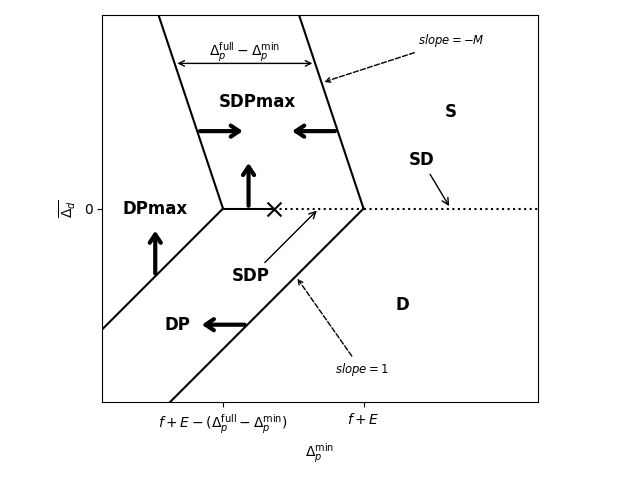
\includegraphics[width=\textwidth]{images/optimal_regime_phase_diagram_Nto0.png}
    \caption{Regimes as $N\rightarrow 0$.}
    \label{fig_diagrammphase_n_to_0}
\end{center}
\end{figure}

\subsubsection{Endogenize $\varphi \in [0, 1]$ as $N \rightarrow +\infty$}

Here, only case j right becomes available, meaning that $N_d /N = \frac{1}{M + 1}$, $N_p / N = \frac{M}{M+1}$ and $\varphi = 1$.

\subsubsection{2 observations for a fixed $\varphi$:}

It is possible to have jumps only if some domains overlap.

It is possible to see a decreasing $N_d$ with $N$. To see that, think of a fixed $\Delta_p$ with $\varphi = 1$. When we jump from $N_p = 0$ to $N_p = \frac{MN}{M+1}$, clearly, $N_d$ decreases

        
        
    \end{itemize}
\end{document}